% --------------------------------------------
% \documentclass[twocolumn]{aastex6}
\documentclass[apj]{emulateapj} %iop
\usepackage{amsmath}


preamble.tex
\slugcomment{To be Submitted}

\makeatletter
\renewcommand\normalsize{\@setfontsize\normalsize\@xpt{12.5}}
% \renewcommand\normalsize{\@setfontsize\normalsize{10.56}{11.4}}      % 11.5, 12.5
\makeatother

\citestyle{aa}
\shorttitle{Dynamical Properties of Molecular Gas Complexes in $z$\ssim6 Prototypical Galaxy
}
\shortauthors{Leung et al.}

\begin{document}
\title{
Dynamical Properties of Molecular Gas Complexes in a Redshift 6 Prototypical Galaxy at the Epoch of Reionization
}


\author{T. K. Daisy Leung\altaffilmark{1, 2}}
\author{Andrea Pallottini \altaffilmark{3, 4}}
\author{Andrea Ferrara \altaffilmark{4, 5}}
\author{Mordecai-Mark Mac Low\altaffilmark{2, 6, 7}}

\altaffiltext{1}{Department of Astronomy, Space Sciences Building, Cornell University, Ithaca, NY 14853, USA}
\altaffiltext{2}{Center for Computational Astrophysics, Flatiron Institute, Simons Foundation, 162 Fifth Avenue, New York, NY 10010, USA}
\altaffiltext{3}{Centro Fermi, Museo Storico della Fisica e Centro Studi e Ricerche ``Enrico Fermi'', Piazza del Viminale 1, Roma, 00184, Italy}
\altaffiltext{4}{Scuola Normale Superiore, Piazza dei Cavalieri 7, I-56126 Pisa, Italy}
\altaffiltext{5}{Kavli IPMU, The University of Tokyo, 5-1-5 Kashiwanoha, Kashiwa 277-8583, Japan}
\altaffiltext{6}{Institut f{\"u}r Theoretische Astrophysik, Zentrum f{\"u}r Astronomie der Universit{\"a}t Heidelberg, 69120 Heidelberg, Germany}
\altaffiltext{7}{American Museum of Natural History, 79th St.~at Central Park West, New York, NY 10024, USA}
\email{tleung@astro.cornell.edu}



\begin{abstract}
We present results from the first study investigating the dynamical properties of molecular clouds 
and their evolution in galaxies at Epoch of Reionization using state-of-the-art cosmological 
zoom-in simulation, which includes a chemical network to determine the formation of molecular 
hydrogen, heating and cooling of the ISM by metals, and stellar feedback via 
kinetic and thermal energies. We..
\end{abstract}
%\keywords{infrared: galaxies --
%          galaxies: high-redshift --
%          galaxies: ISM --
%          galaxies: evolution --
%          galaxies: starburst --
%          radio lines: ISM}


\def\figpath{./Fig}

%--------------------------------------------------------------------------
%                                Introduction
%--------------------------------------------------------------------------
\section{Introduction}    \label{sec:intro}

The growth of galaxies and their subsequent evolution are governed by the baryonic/baryon cycle ---
galaxies accrete gas from the intergalactic medium to fuel \SF (and feed their supermassive blackholes)
and subsequent feedback replenishes and enriches the circumgalactic medium with part of this material.
The general consensus is that the growth of \highz galaxies are triggered/supported by massive
gas inflows from mergers and/or the cosmic web at early cosmic time, when the intergalactic 
medium and galaxies themselves are more gas-rich in their star-forming molecular 
gas contents compared to present-day galaxies.
 % while at a given snapshot, the gas mass fraction maybe low (esp. at high-z when 
% the gravitational potential is still increasing), but their gas reservoirs 
% are continuously being replenished. 
These massive gas inflows in turn trigger gravitational instability, and thus, lead
to the formation of clouds/structures that are typically more massive and denser than those 
observed in nearby galaxies, with cloud masses of $M_{\rm cloud}$\eq10$^9$\,\Msun 
and sizes on sub-kpc scales (e.g. \citealt{Gabor13a, Hopkins14a, Inoue16a}).
%In cosmological context, minor mergers and external gas accretion can
%significantly impact on disc dynamics and clump formation
%(e.g. Bird et al. 2012, MNRAS, 420, 913; Kyziropoulos et al. 2016, MNRAS, 463, 2210).
Some theoretical works postulate that it is in fact the
migration of such giant massive clumps that are responsible for contributing to the 
buildup of the bulges of massive galaxies at \z$\sim$0 \citep[e.g.,][]{Ceverino10a}.


At high redshifts, galaxies are expected to have lower metallicity, 
% stronger and harder radiation fields),
more {\sc HII} regions and ionized gas 
(given their much higher star formation rates; SFR), and 
more intense radiation stellar feedbacks.
Such differences in turn affect the thermal and chemical structures of their ISM (e.g., shielding of UV photons, heating and cooling mechanisms, and elemental abundances),
and thus, their multi-phase ISM differ from nearby galaxies.
Since \highz galaxies are the early stages of evolution of present-day galaxies, 
studying their ISM properties is essential for understanding how \SF proceed under these more extreme
conditions, thereby driving the evolution and assembly history 
of galaxies since the cosmic dark ages.
% since they set the pace for chemical reactions and excitation rates for the coolants in the ISM (and subsequent star formation). 

The FIR fine-structure lines (e.g., \cii, \nii, and \oiii), and CO/[\ci]~lines are the key diagnostics for 
constraining the ISM conditions of galaxies and
provide highly complementary information tracing the different phases of the ISM (ionized, 
atomic, molecular; e.g., \citealt{Scoville74a, Rubin85a, Malhotra01a}).
Global measurements of these diagnostics in \highz galaxies 
have informed us on their galaxy-wide properties (e.g., 
gas masses, gas temperature, and radiation field intensity).
However, spatially resolving their ISM is needed in order to understand their role in galaxy evolution and 
the physics behind their intense \SF (SFR\ssim100$-$3000\,\Msun\,yr\pmOne).
To date, the ISM properties of \highz galaxies 
have only been studied observationally in a handful of (strongly-lensed) 
galaxies, using spatially resolved tracers such as 
dust continuum, and CO and \cii lines (e.g., \citealt{Swinbank11a, Hodge15a, Ferkinhoff15a, Hodge16a},
Leung et al. 2018, submitted).
These studies find that the ISM of $z$\ssim2 galaxies are more 
molecular gas-rich, turbulent, and clumpy than nearby galaxies.
However, it is still unclear how \SF proceed in the (sub-)$L^*$ galaxy population at \z$\gtrsim$\,6 
that dominates  \SF at the epoch of reionization which is responsible for producing the 
ionizing photons that reionized the universe.

While ALMA has enabled the detections of 
ISM diagnostic lines e.g., the \cii158\,$\micron$ and CO line emission in 
normal (SFR$<$\,100\,\Msun\,yr\pmOne) galaxies at \z$>$\,6 over the past few years \citep[e.g.,][]{Smit18a},
we are still far from mapping their molecular ISM.
In particular, their star-forming gas conditions, due to the stupid stingy ALMA TAC.
As such, we have undertaken a study, exploiting 
state-of-the-art cosmological zoom-in hydrodynamic simulation 
\ncode{Serra} (Greenhouse in Italian; \citealt{Pallottini17a, Pallottini17b}), to examine 
the dynamical properties of the molecular cloud complexes in a \z$\sim$6 prototypical (i.e., $L^*$) lyman-break
galaxy (LBG).

This paper is structured as follows.
In \Sec{sim}, we describe the setup of our simulation and the properties of our galaxy (\flower).
In \Sec{method}, we describe the method used to identify its molecular gas complexes (MC). 
In \Sec{results}, we present scaling relations found based on the properties of 
the identified MC and compare them with observations of molecular 
(sub-)structures seen in nearby and \z$>$\,0 galaxies.
In \Sec{diss}, we discuss the results and implication of our findings,
and conclude in \Sec{conclusion}.
Throughout this paper, we adopt a concordance cosmology, with total matter, vacuum and baryonic densities 
in units of the critical density $\Omega_{\Lambda}$\eq0.692, $\Omega_m$\eq0.308, $\Omega_b$\eq0.0481, 
Hubble constant $H_0$\eq100\,$h$\,km s\pmOne\,Mpc\pmOne with $h$\eq0.678, 
spectral index $n$\eq0.967 and $\sigma_8$\eq0.826 \citep{Planck14a}.


% ------------------
\section{Simulations} \label{sec:sim}

\subsection{\ncode{Serra} Simulation\footnote{Serra means greenhouse in Italian which is motivated by the
fact that our simulation includes a chemical network to calculate the abundance of H$_2$, which in turn 
dictates the formation of CO.
}}  
The simulation used in this work is described by \citealt{Pallottini17a} and is briefly summarized here.

\ncode{Serra} is a cosmological zoom-in simulation performed using Eulerian hydrodynamics and 
adaptive mesh refinement (AMR) technique to achieve high spatial resolution in the region of interest (i.e., regions of high baryonic density).
In particular, it uses a modified version of \ncode{ramses} as the AMR backend.
\ncode{Serra} uses sub-grid models that simultaneously account for the radiative transfer, clumpy structure, and 
photoevaporation feedback in the neutral diffuse and molecular gas. 
Our simulation covers a co-moving box of 20\,Mpc $h$\pmOne in size, resolving 
down to a physical scale of 30\,pc (at \z$\sim$\,6) and a (baryonic) mass resolution of $m_b\simeq$\,10$^4$\,\Msun in the 
finest level.
Such a physical scale is close to the size scale of molecular cloud complexes and
giant molecular clouds (GMCs), as seen in nearby galaxies \citep[e.g.,][]{Sanders85a, Federrath13a, Goodman14a}.
% (Giant molecular clouds: L>22pc, m>10^5 Msun) in MW.
We include chemical network in the simulation to trace 
$\rm{H}$, $\rm{H}^{+}$, $\rm{H}^{-}$, $\rm{He}$, $\rm{He}^{+}$, $\rm{He}^{++}$, $\rm{H}_2$, $\rm{H}_2^{+}$ \citep{Grassi14a,Bovino16a}.
Of particular importance to our study here is that 
our simulation includes non-equilibrium formation of molecular 
hydrogen (done on-the-fly) to determine the H$_2$ abundance (see \citealt{Pallottini17b} for effects of 
chemistry affected by non-equilibrium versus equilibrium H$_2$ formation). 
Star formation is modeled using a H$_2$-based prescription of the Schmidt-Kennicutt relation \citep{Krumholz09a}.
We adopt stellar tracks from \ncode{starburst99} and 
include stellar feedback from supernova, OB/AGB stars to account for energy dissipations.
The energy dissipated is then injected into the ISM in the form of kinetic and thermal energy.
Radiation pressure (on the dust and gas) is also included.  % radiative feedback --> NT pressure
To couple the feedback to the gas, we 
employ sub-grid modeling for blastwaves to account for the potential lost of energy inside the cell when
supernovae are exploded.

Details of how \flower, the main galaxy in our simulation,
was identified is discussed in detail by \citet{Pallottini17a}.
Briefly, by \z$\sim$6, \flower is a LBG hosted in 
a dark matter halo of mass $M_{\rm DM}\simeq$\,10$^{10}$\,\Msun at the center of a cosmic web knot, and 
accretes mass from the intergalactic medium mainly via three filaments of length $\simeq$\,100\,kpc.
At \z$\sim$6, \flower has a stellar mass of $M_*\simeq$\,3\E{10}\,\Msun,
metallicity of $Z\simeq$\,0.5\,$Z_{\odot}$,
a molecular gas mass of $M_{\rm H2}\simeq$\,5\E{7}\,\Msun,
and a globally-integrated SFR of $\simeq$\,100\,\Msun\,yr\pmOne\footnote{This includes contributions from its nearby massive satellite galaxies.}.
It is therefore a prototypical galaxy at \z$\sim$6.



\section{Method} \label{sec:method}

To identify the molecular complexes, we use a customized version of the clump finder algorithm 
available in the \ncode{python} package \ncode{yt}, which was initially described in \citet{Smith09a}
but this function has been modified since then.
The latest version of the default \ncode{yt} clump finder decomposes the cells in the simulation
into non-overlapping tiles, which are stored in a k-dimentional tree (aka k-d tree).
It then identifies the contours of a variable field (e.g., density field) within a tile and connects them across 
the tiles. In the customized version used for this study, we modified \ncode{yt} in order for it to actually work.

In the ``clump-finding'' process, we employ a set of different density thresholds defined based on the
molecular hydrogen density of \flower taken at different cosmic times (between $z$\eq6\,$-$\,15, {\bf Pallo, check this pls}).
We note that this process is in essence similar to 
identifying molecular structures based on the noise levels of surface density maps 
observers obtain with telescopes, using molecular line tracers such as CO, CS, and HCN,
as commonly adopted in observational studies (e.g., identifying 
``clumps'' based on/after applying $\sigma$-clipping, 
using tools such as \ncode{aips}'s task \ncode{serch}, \ncode{clumpfind}, 
and \ncode{cprops}; \citealt{Williams94a, Rosolowsky06a}).


\begin{figure}[htbp]
\centering
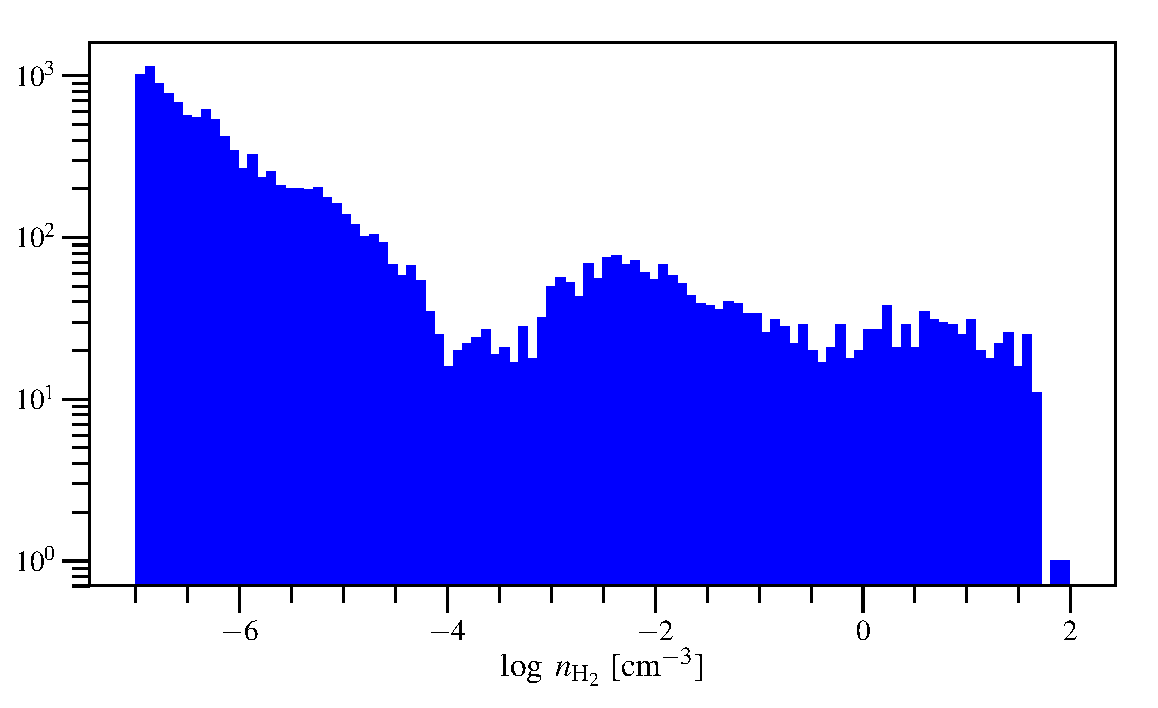
\includegraphics[trim=35 0 10 35, clip, width=0.55\textwidth]{\figpath/hist_test_16.pdf}  
\caption{
Volumetric H$_2$ density distribution of \flower taken from a single snapshot.
\label{fig:h2density}}
\end{figure}


\begin{figure*}[htbp]
 \centering
  \includegraphics[scale=0.7]{\figpath/{dual_16_ncut_0.32}.png} 
  \\[-5.5em]
  \includegraphics[scale=0.7]{\figpath/{dual_16_ncut_0.53}.png} 
\caption{
MC identified by applying 
volumetric H$_2$ density cuts of 
$n_{\rm cut}$\eq[0.32, 0.53, 0.88, 1.45, 2.45, 4.08, 6.81, 11.36, 19.00, 31.62]\,cm$^{-3}$.
Color shows the projected H$_2$ surface density. {\bf this should be H2 density 1/cm$^{-2}$?!}
% yt.OffAxisProjectionPlot: weight the requested field by the weighting field and integrate along the line of sight.
\label{fig:MC}}
\addtocounter{figure}{-1}
\end{figure*}

\begin{figure*}[htbp]
 \centering
  \includegraphics[scale=0.7]{\figpath/{dual_16_ncut_0.88}.png}
    \\[-5.5em]
  \includegraphics[scale=0.7]{\figpath/{dual_16_ncut_1.47}.png}
\caption{
Continued.}
\addtocounter{figure}{-1}
\end{figure*}

\begin{figure*}[htbp]
 \centering
  \includegraphics[scale=0.7]{\figpath/{dual_16_ncut_2.45}.png}
  \\[-5.5em]
  \includegraphics[scale=0.7]{\figpath/{dual_16_ncut_4.08}.png}
\caption{
Continued.}
\addtocounter{figure}{-1}
\end{figure*}

\begin{figure*}[htbp]
 \centering
  \includegraphics[scale=0.7]{\figpath/{dual_16_ncut_6.81}.png} 
  \\[-5.5em] 
  \includegraphics[scale=0.7]{\figpath/{dual_16_ncut_11.36}.png}
\caption{
Continued.}
\addtocounter{figure}{-1}
\end{figure*}

\begin{figure*}[htbp]
 \centering
  \includegraphics[scale=0.7]{\figpath/{dual_16_ncut_18.96}.png} 
  \\[-5.5em]  
  \includegraphics[scale=0.7]{\figpath/{dual_16_ncut_31.62}.png} 
\caption{
Continued.}
\end{figure*}

In \Fig{h2density}, we show an example of the volumetric H$_2$ density distribution of \flower 
for a given snapshot which includes contributions from its surrounding 7\,kpc.
In \Fig{MC}, we show an example of
the molecular structures identified by applying volumetric H$_2$ density cuts of 
$n_{\rm cut}$\eq[0.32, 0.53, 0.88, 1.45, 2.45, 4.08, 6.81, 11.36, 19.00, 31.62]\,cm$^{-3}$\footnote{
Based on 10$^n$, where $n$ represents the 10 elements that are 
uniformly spaced between [$-0.5, 1.5$] in linear space.
We also vary the range of 
$n_{\rm cut}$ adopted and find no significant differences 
affecting the results and conclusions of this work (see \Sec{ncut}).}
to the same snapshot as that 
used to plot \Fig{h2density}.
Since the molecular structures identified could 
easily appear as overlapping structures depending on the viewing angle, we 
also plot them in different three-dimensional projections --- so that one can more 
easily see that they are collections of disjoint structures.
We repeat this identification process for 14 snapshots, spaced by $\Delta t$\eq50\,Myr. 
{\bf TODO: 0.1\,Myr (500 snapshots at $z$\eq9)}
Limited by the spatial resolution of our simulation ($l_{\rm cell}\simeq$\,30\,pc), we 
impose an addition constraint such that an identified structure only survives if it
spans at least 10 cells in 3D position-position-position (PPP) space. 
We caution that one caveats of such constraint is that 
we can only examine the parameter space of ``cloud'' scaling
relations at ``cloud'' size $R\gtrsim100$\,pc. 



% --------------------
\section{Star Formation History and Cloud Evolution} \label{sec:sfh}

One of the advantage of studying the dynamical properties of molecular structures at 
$z$\ssim6 in simulation is the fact that we can examine how their properties evolve 
as a function of time. 
Especially at early epochs, where the densest structures are beginning to form; 
gas is constantly being accreted onto the central galaxy from the cosmic web and 
satellite galaxies, thereby leading to bursts of \SF.
Meanwhile, tidal forces resulting from interactions with these surrounding 
galaxies can disrupt the main disk and arms, likely leading to different dynamical states 
for the molecular structures (e.g., some may disperse, some may agglomerate into more massive 
structures). % mainly expecting differences in alpha_vir, sigma, M_cl.

We show the \SF history of \flower in \Fig{SFH}, where 
the SFR of \flower varies between $\sim$30$-$80\,\Msun\,yr\pmOne\footnote{
The SFR plotted in Figure 2 of \citet{Pallottini17b}
is a factor of two higher than shown here since they also include contributions from 
massive satellites galaxies within the surrounding xxx\,kpc.}
as it evolves from an actively accreting phase to 
a starburst phase after a major merger and then back to a relatively quiescent phase
over the few hundred Myr simulated in our simulation.
The SFR of \flower is calculated based on existing young stellar population, which is 
defined to have an age of $t_{\rm age}<$\,10\,Myr.

Given the stochasticity in the \SF history of \flower, 
we show the scaling relations found for two particular snapshots as examples in \Sec{singless},
since they represent the extreme evolutionary stages of \flower (and thus, likely bracket the
most extreme variations in the cloud dynamics) --- one of which \flower is 
actively accreting materials from its surrounding (top panel of \Fig{phases}) 
and another of which \flower is undergoing 
a starburst phase after a major merger (bottom panel of \Fig{phases}). 



\begin{figure*}[htbp]
\centering
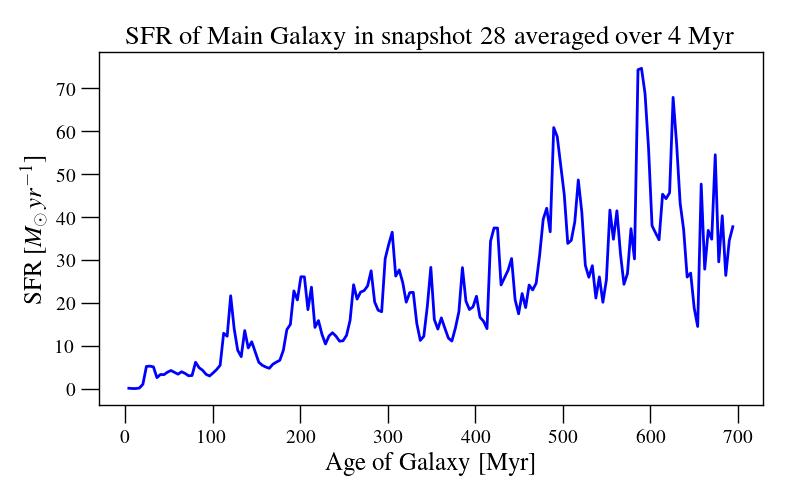
\includegraphics[trim=0 0 0 23, clip, width=0.45\textwidth]{\figpath/snapshot28_SFR_4Myr.png}  
\caption{
Star formation history of \flower.
\label{fig:SFH}}
\end{figure*}


\begin{figure}[htbp]
\centering
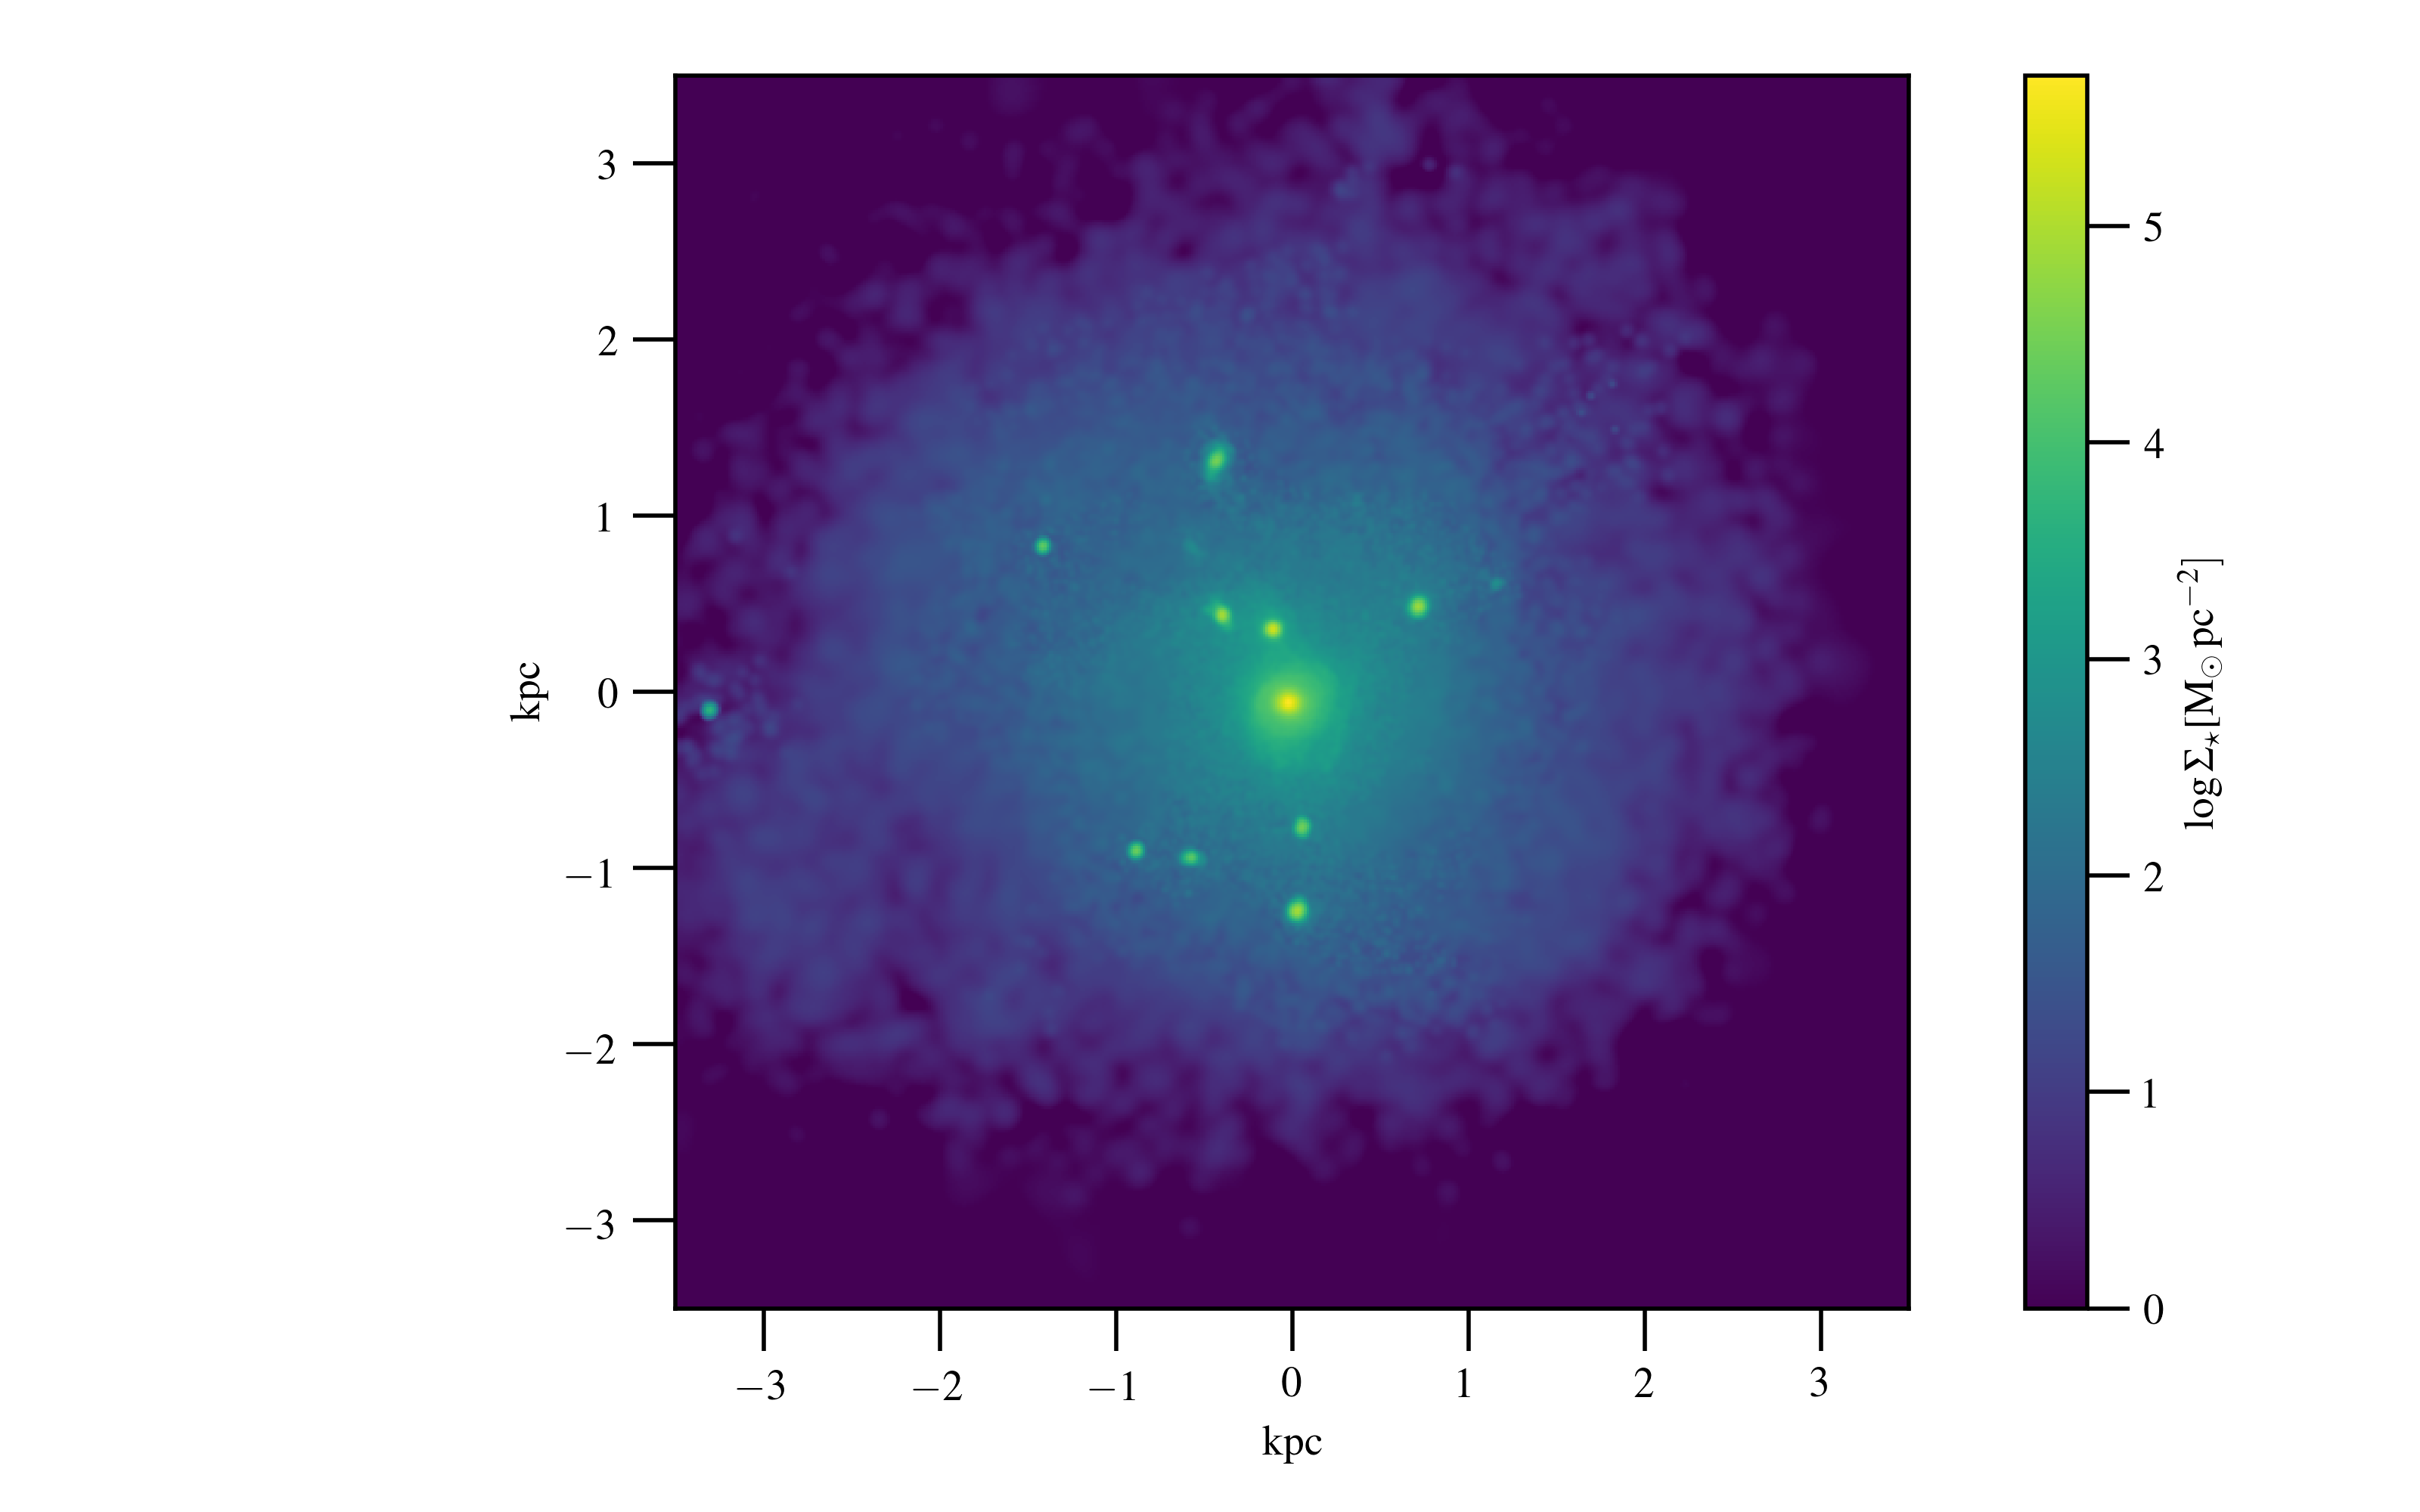
\includegraphics[trim=120 0 0 0, clip, width=0.55\textwidth]{\figpath/star_16.png}  
\\ [-5em]
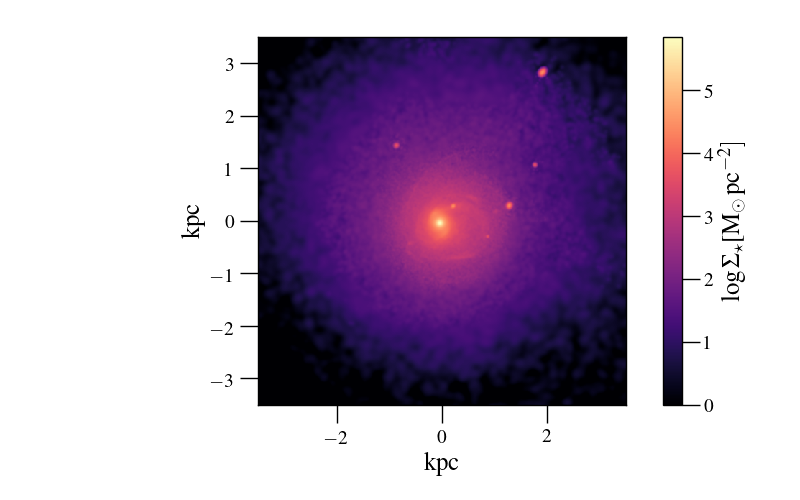
\includegraphics[trim=120 0  0 0, clip, width=0.55\textwidth]{\figpath/star_27.png}  
\caption{
Projected stellar mass distribution of \flower during one of its accretion phases 
at an early stage of its evolution (top) and during one of its major starburst phases 
after a major merger (bottom).
\label{fig:phases}}
\end{figure}

\section{Cloud scaling relations} \label{sec:results}
Upon identified the molecular structures, we extract parameters such as
the virial parameter ($\alpha_{\rm vir}$), 
the cloud mass ($M_{\rm cl}$), 
the Mach number ($\mathcal{M}$), 
the velocity dispersion ($\sigma_v$), and the 
gas surface density ($\Sigma_{\rm gas}$)
to describe/characterize their dynamics.
We find that the thermal sound speed ($c_s$) 
of all identified molecular complexes are generally much smaller compared to the their
turbulent velocities.
We find comparable velocity dispersion derived by taking the root mean square ($\sigma_v^{\rm rms}$) versus
that derived using thermal and non-thermal pressure ($\sigma_v^{P+P_{\rm nt}}$), indicating that 
rotation velocity is unlikely to be the dominant source entering the velocity dispersion reported here.
In the subsequent sections, we adopt the root mean square of the velocity field
as the velocity dispersion (i.e., $\sigma_v$\eq$\sigma_v^{\rm rms}$).

\subsection{Single snapshots}  \label{sec:singless}
In each snapshot (see \Fig{MC} for example), 
we identify a set of MCs with consistently high turbulences and surface densities 
regardless of the H$_2$ density cuts adopted. 
These are the MCs at the center of the main disk of \flower.
Their high velocity dispersions and surface densities are expected since 
they are located in the nuclear regions of the 
galaxy, where the potential well is also deeper.

As we increase the density threshold, some of the MC within the main disk break 
into multiple sub-MCs.
As such, we effectively identify a population of denser molecular structures. 
This population of sub-MCs has dynamics largely
similar to those observed 
in $z$\ssim2 spatially resolved studies of gas-rich SFGs, in
terms of their velocity dispersions, sizes, and gas surface densities \citep[e.g.,][]{Swinbank11a}.

We also identify MCs in the satellite galaxies of \flower. These MCs 
tend to have lower virial parameters compared to the (sub-)MCs in the main disk of \flower, 
with $\alpha_{\rm vir}\simeq$1.
Given their low $\alpha_{\rm vir}$ parameter,
these structures are likely collapsing structures (\Fig{alpha16}). 


\begin{figure*}[htbp]
\centering
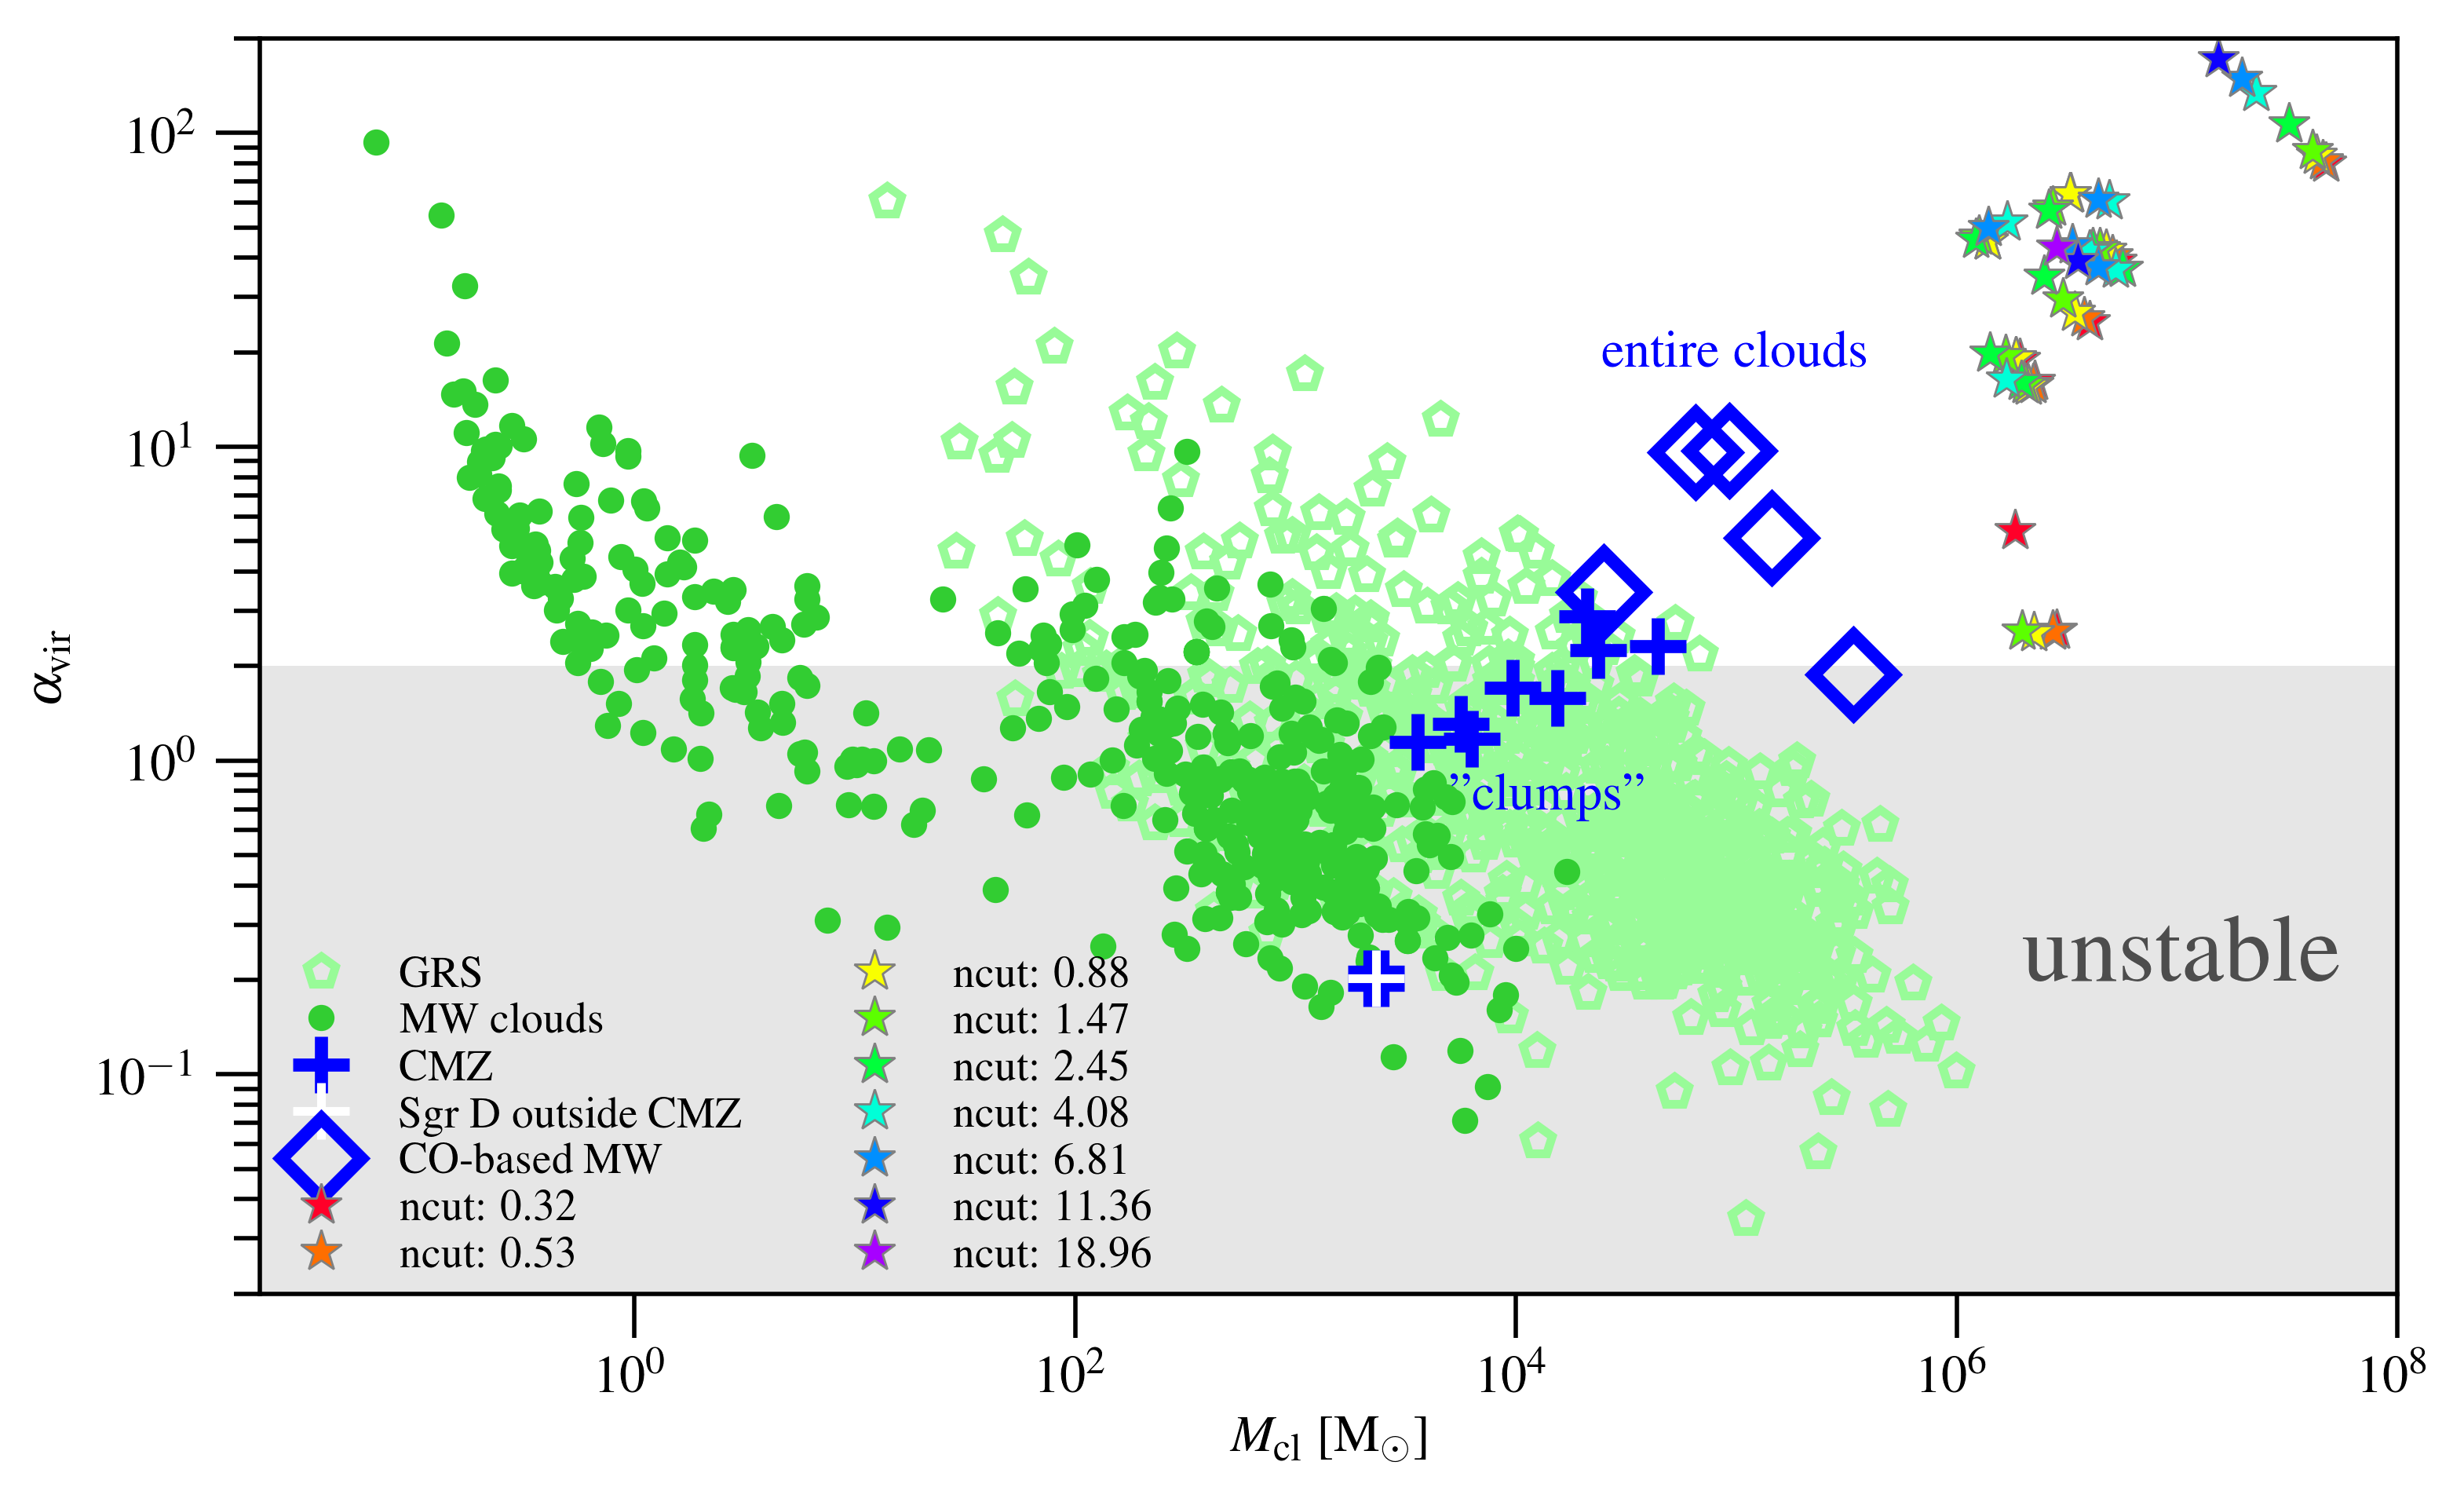
\includegraphics[trim=0 0 0 0, clip, width=0.85\textwidth]{\figpath/ss16_alphavir.png}  
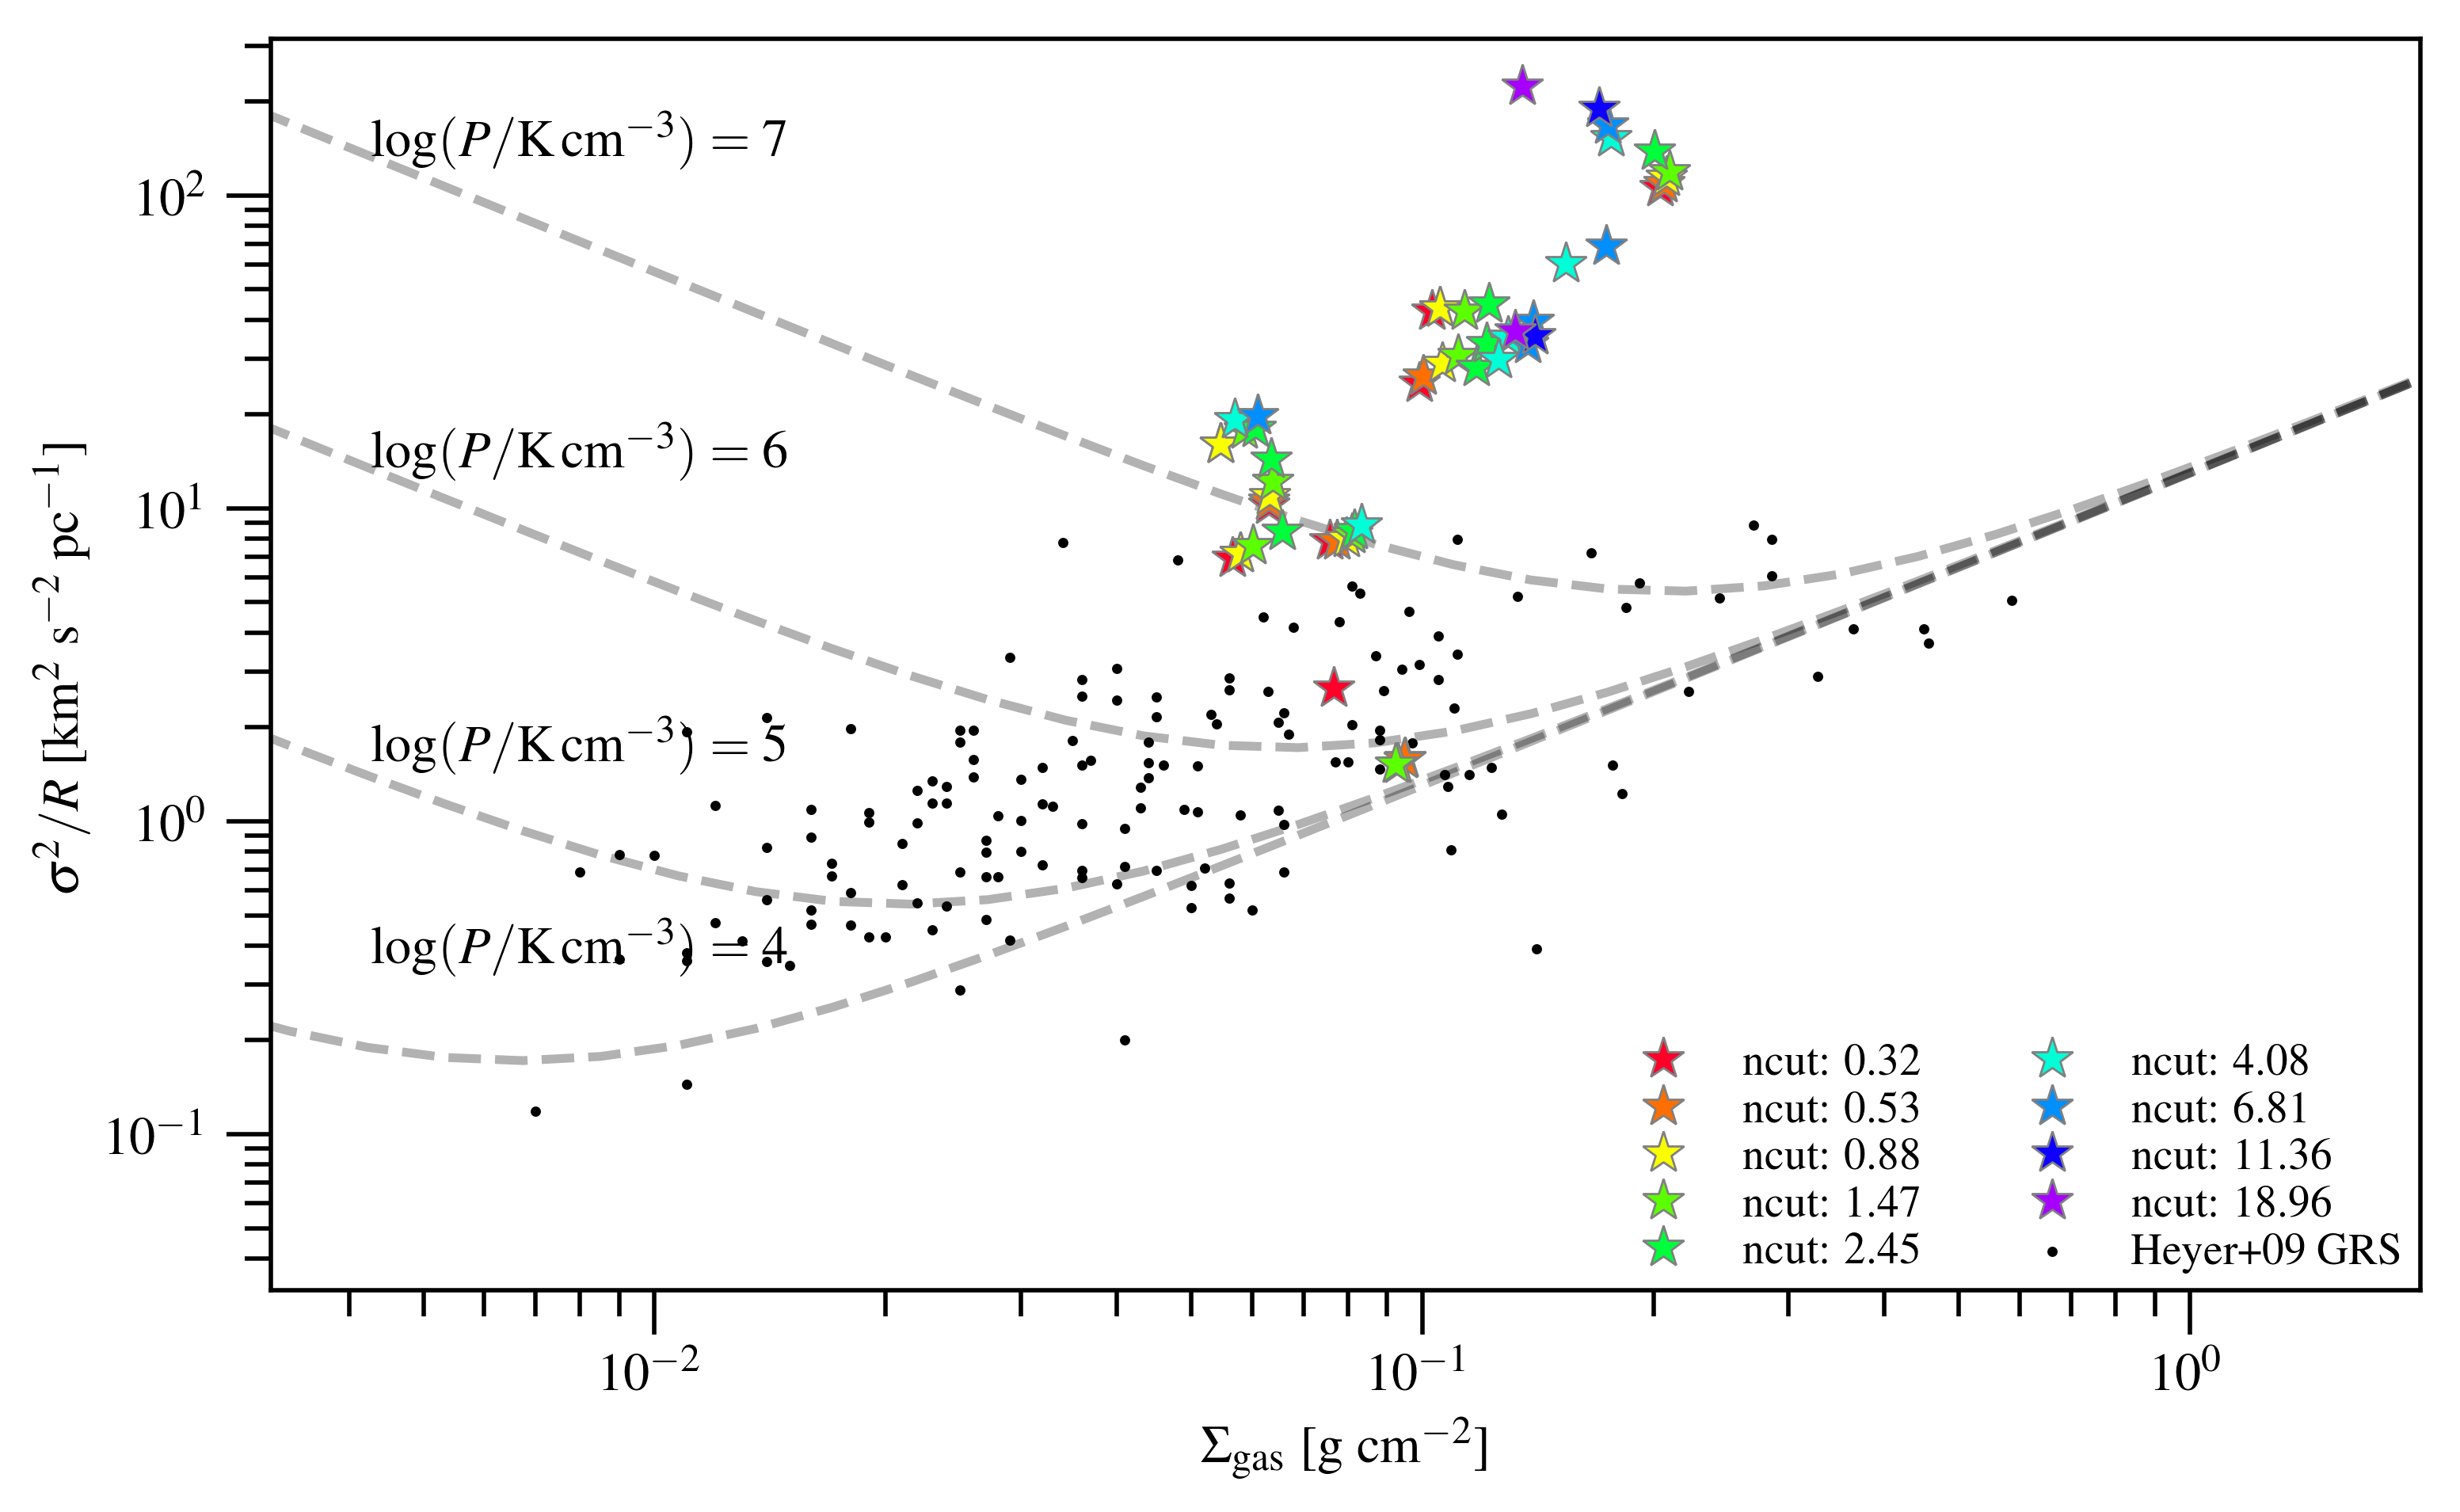
\includegraphics[trim=0 0 0 0, clip, width=0.85\textwidth]{\figpath/ss16_PVE.png}
\caption{
Top: Virial parameter and cloud mass of \flower of a given snapshot (accreting phase).
Bottom: $\sigma^2/R - \Sigma_{\rm gas}$ relation of MCs in the same snapshot.
\label{fig:alpha16}}
\end{figure*}


\begin{figure*}[htbp]
\centering
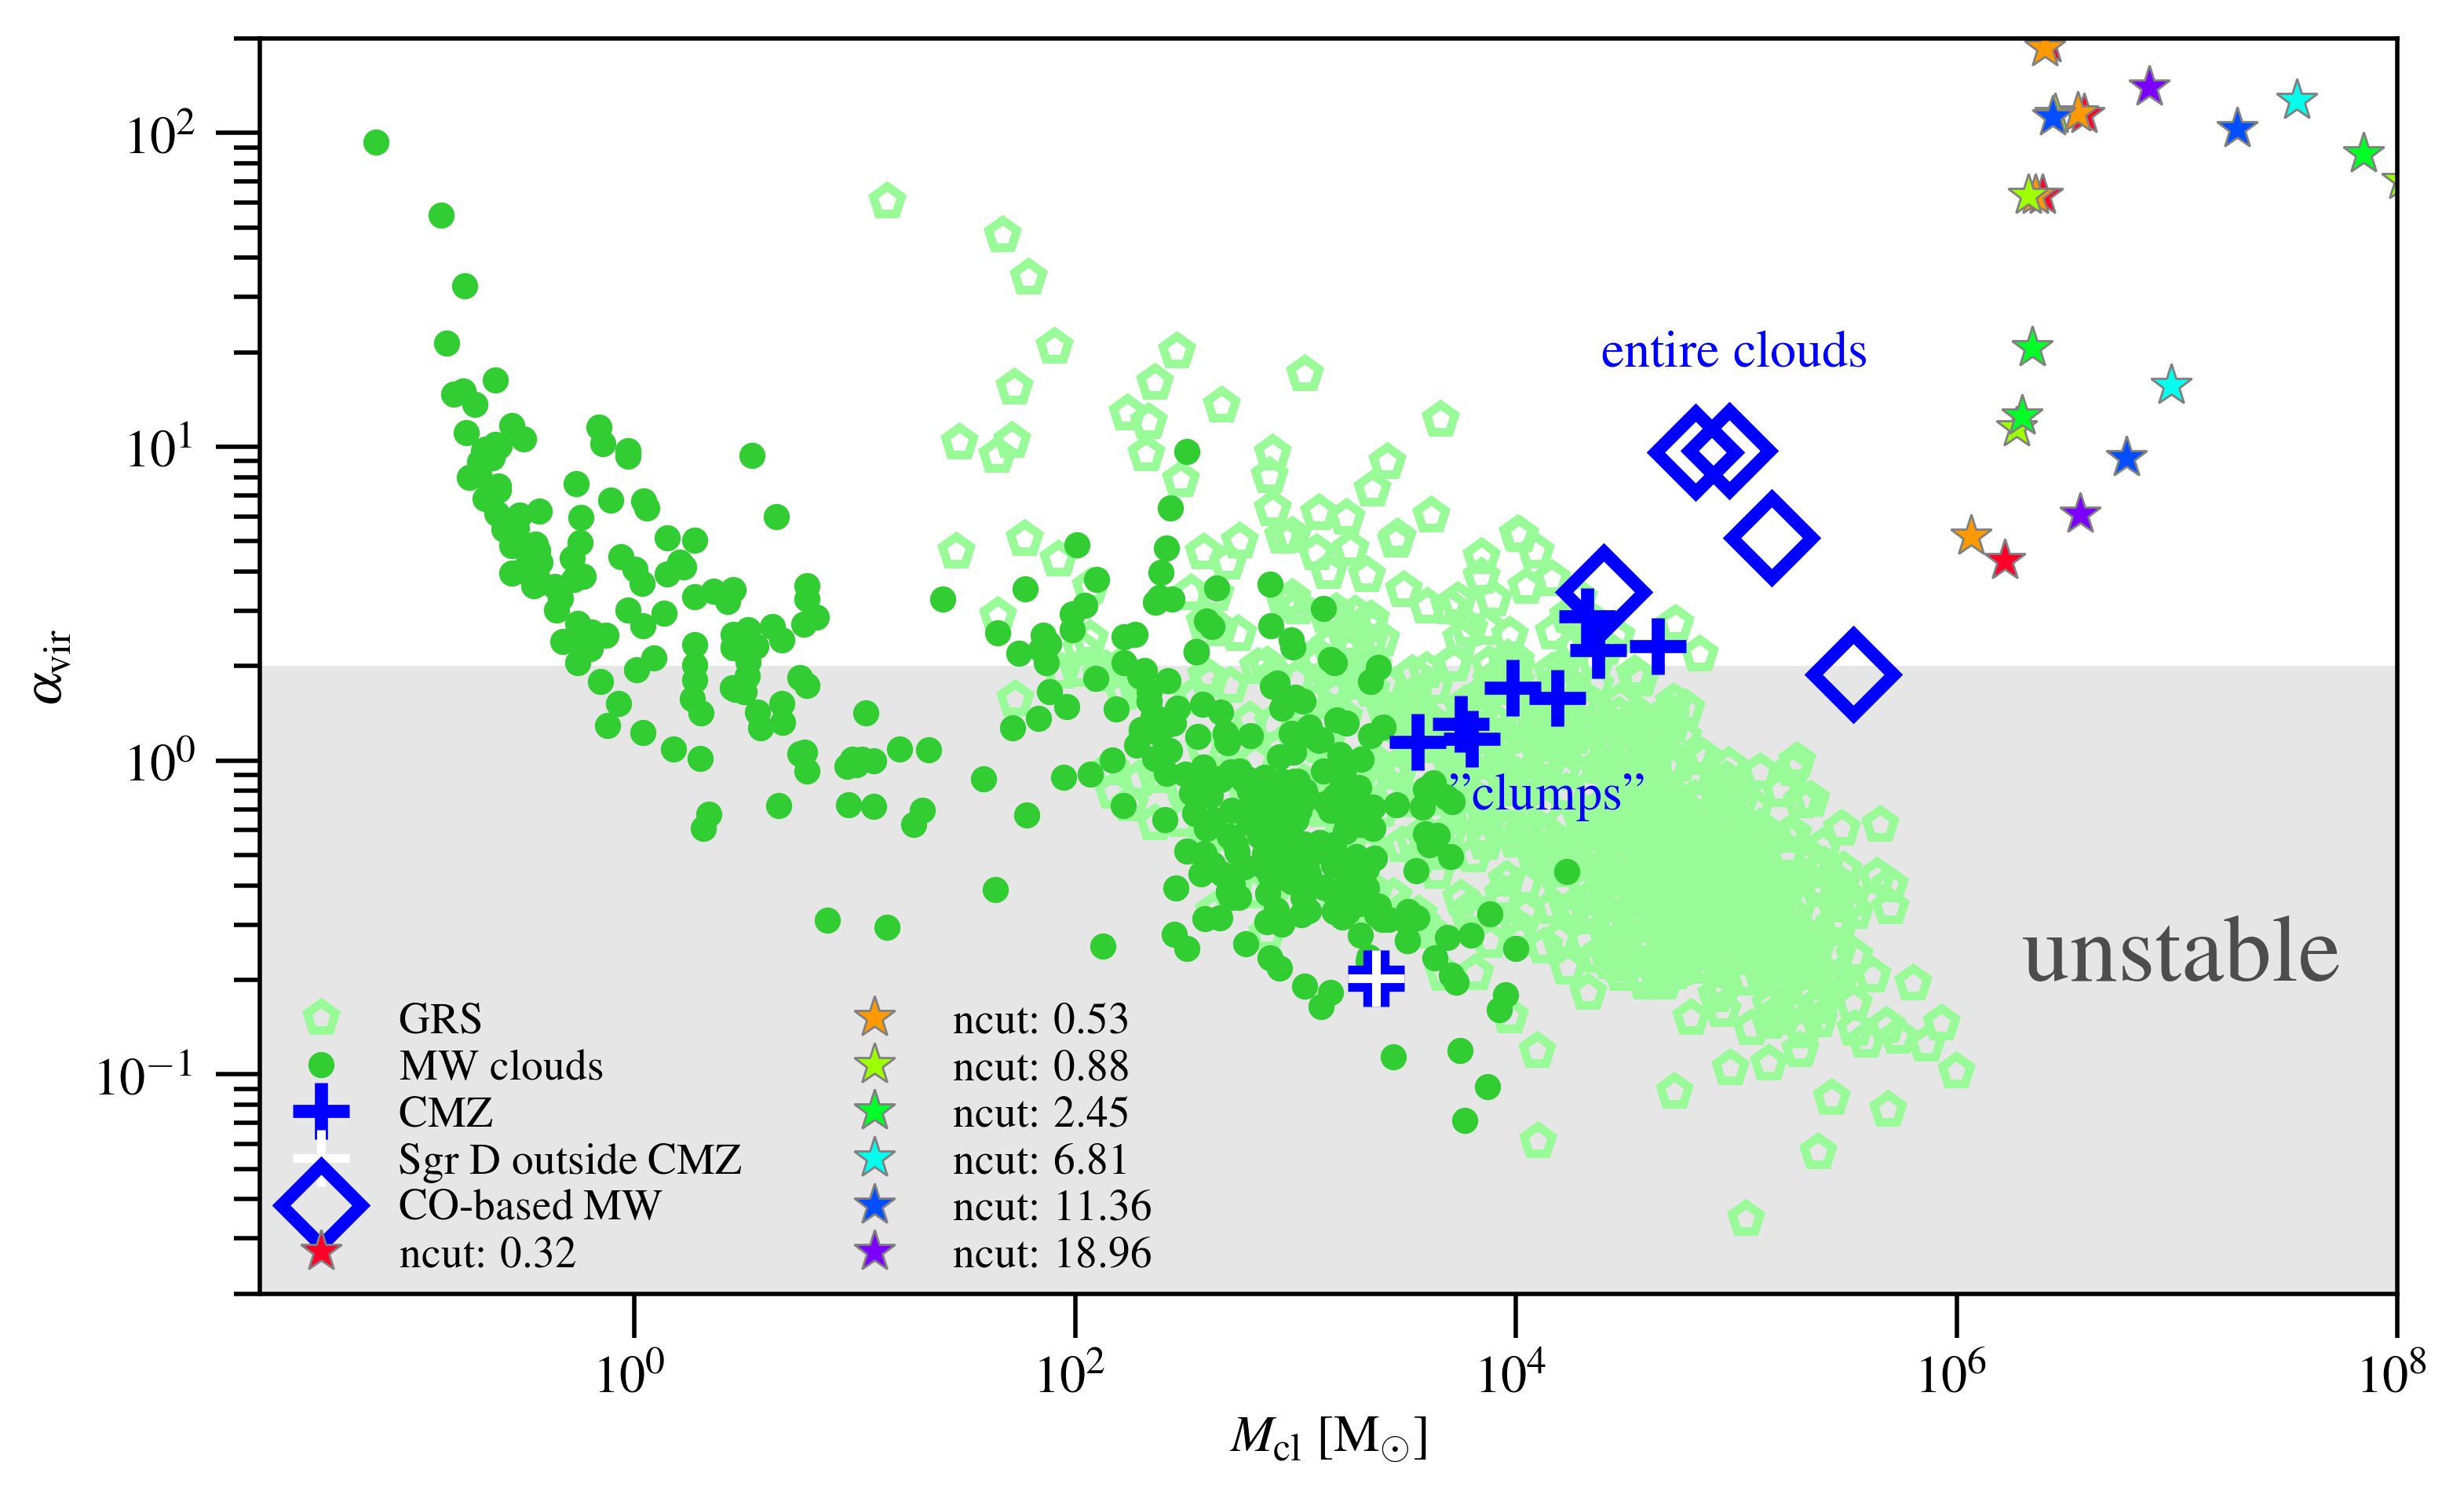
\includegraphics[trim=0 0 0 0, clip, width=0.85\textwidth]{\figpath/ss27_alphavir.png}  
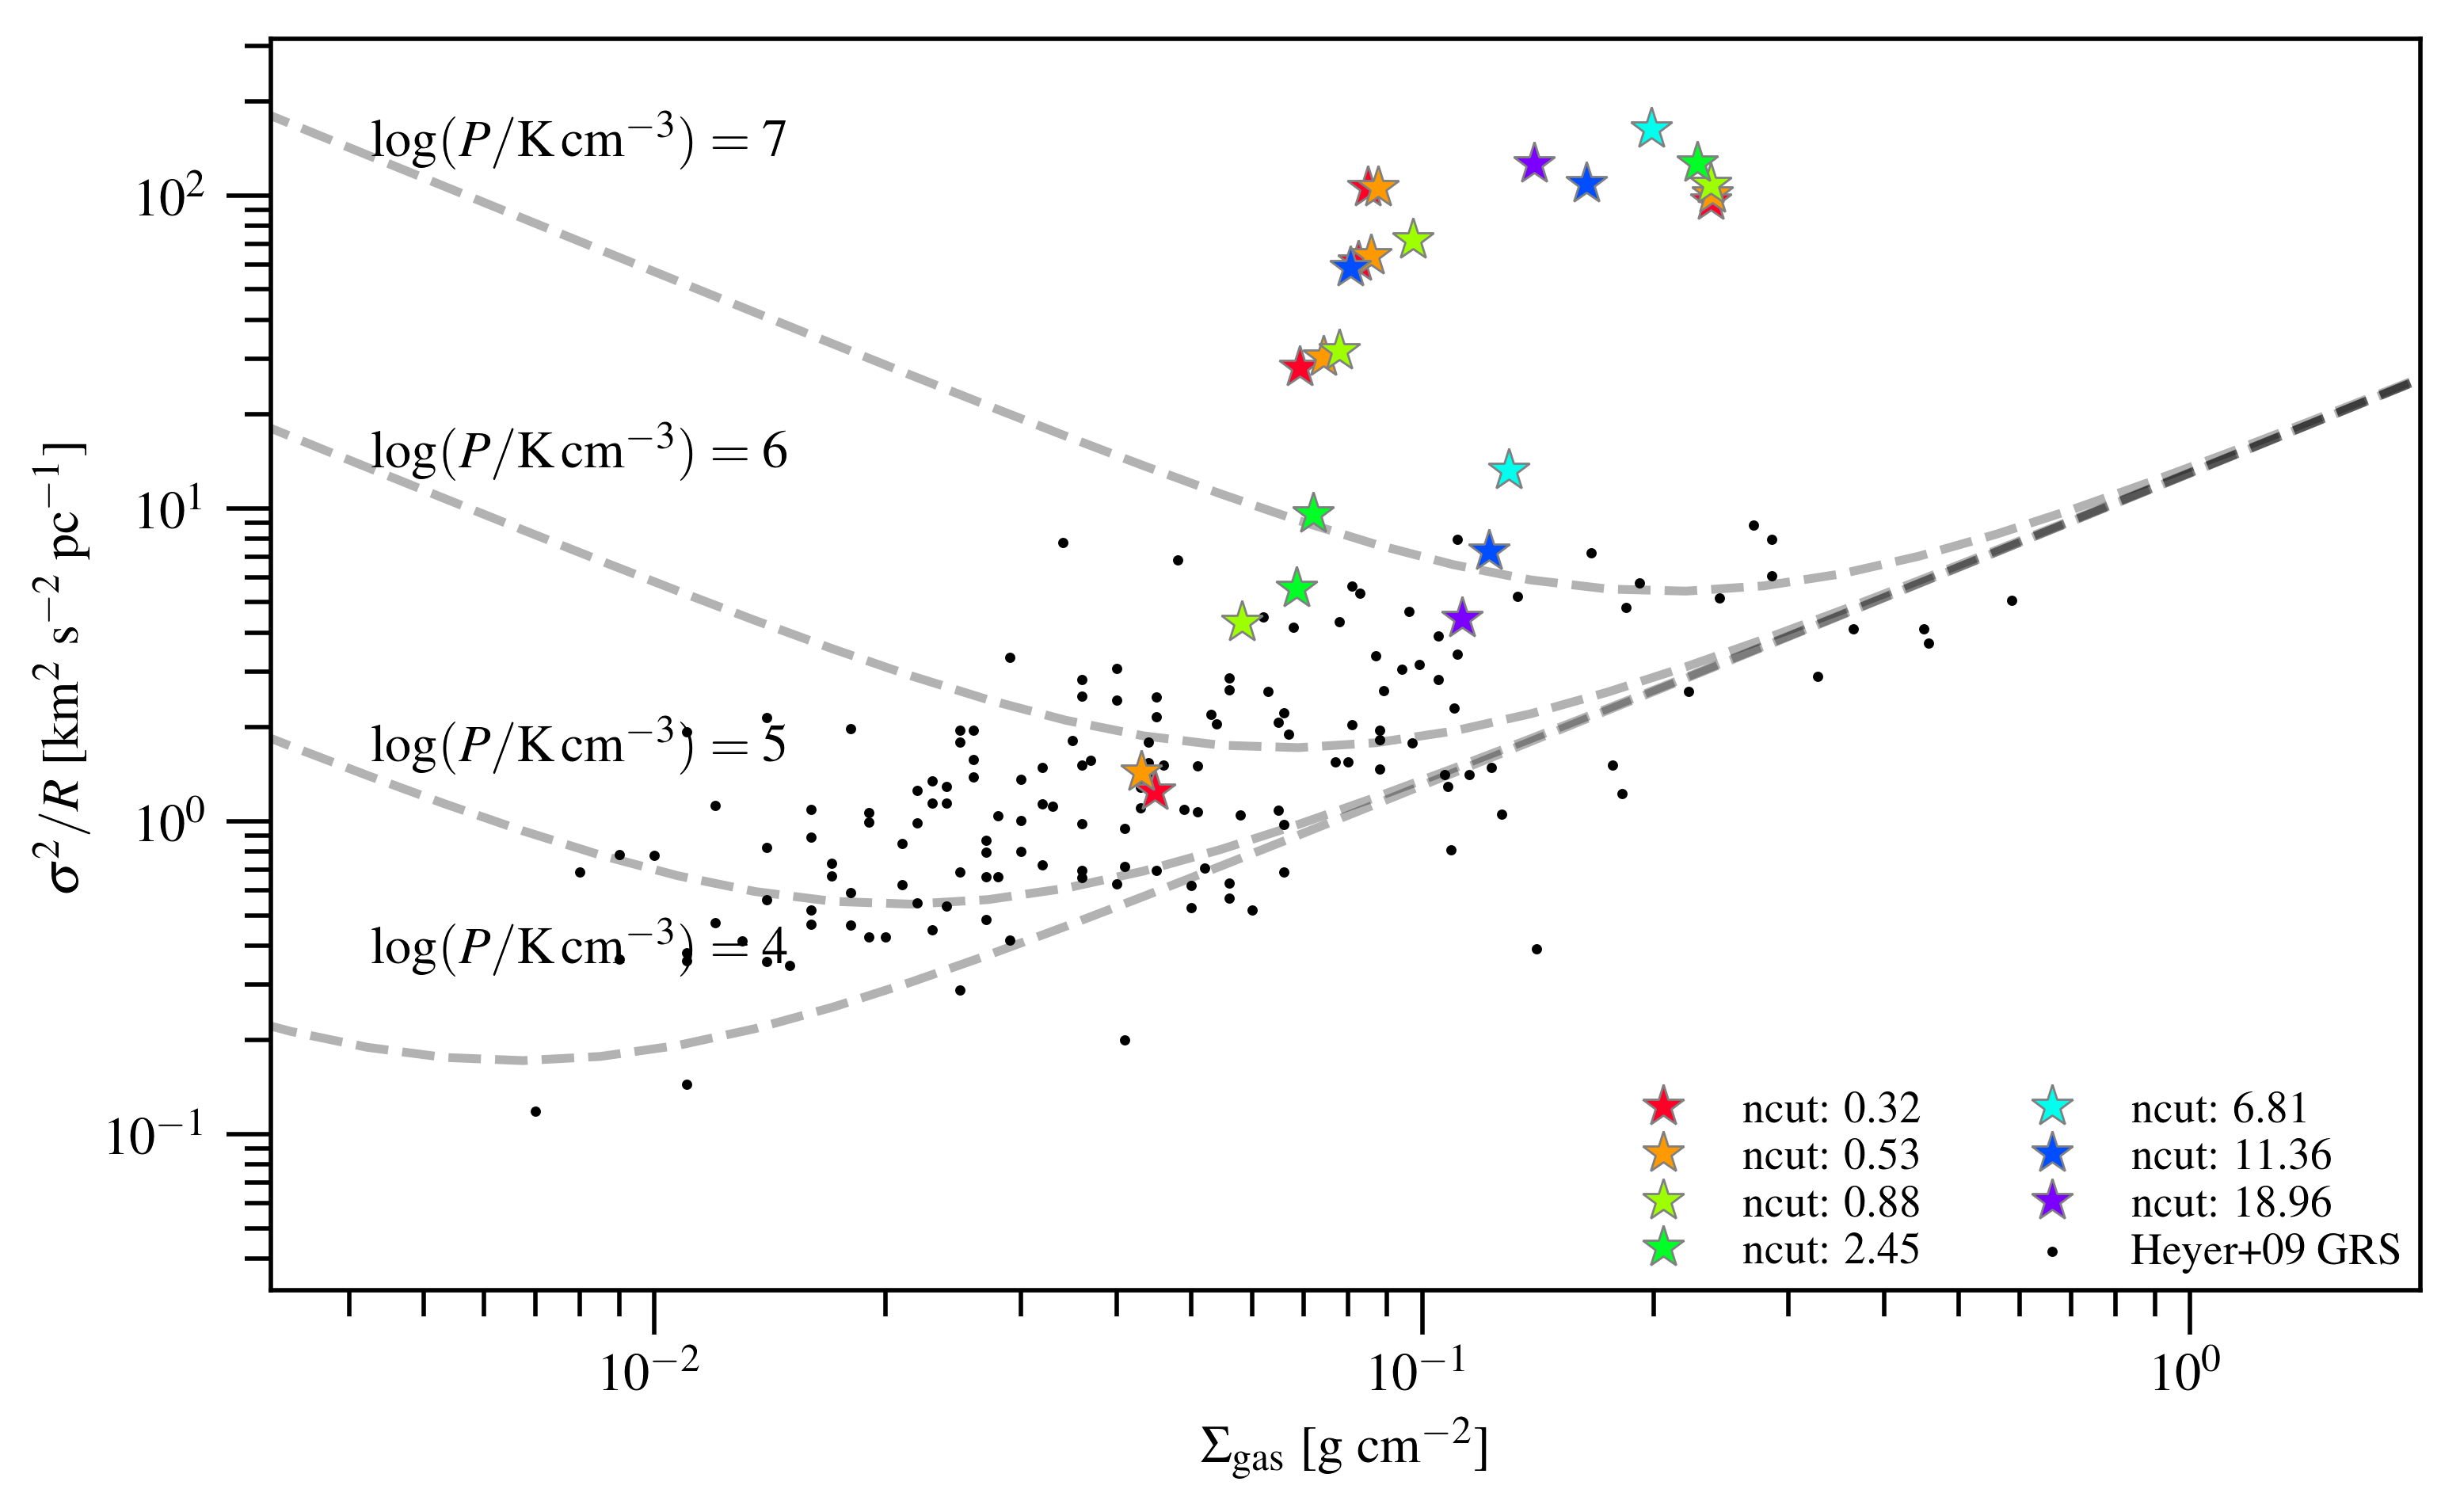
\includegraphics[trim=0 0 0 0, clip, width=0.85\textwidth]{\figpath/ss27_PVE.png}
\caption{
Top: Virial parameter and cloud mass of \flower of a given snapshot (starburst phase).
Bottom: $\sigma^2/R - \Sigma_{\rm gas}$ relation of MCs in the same snapshot.
\label{fig:alpha27}}
\end{figure*}

\begin{figure*}[htbp]
\centering
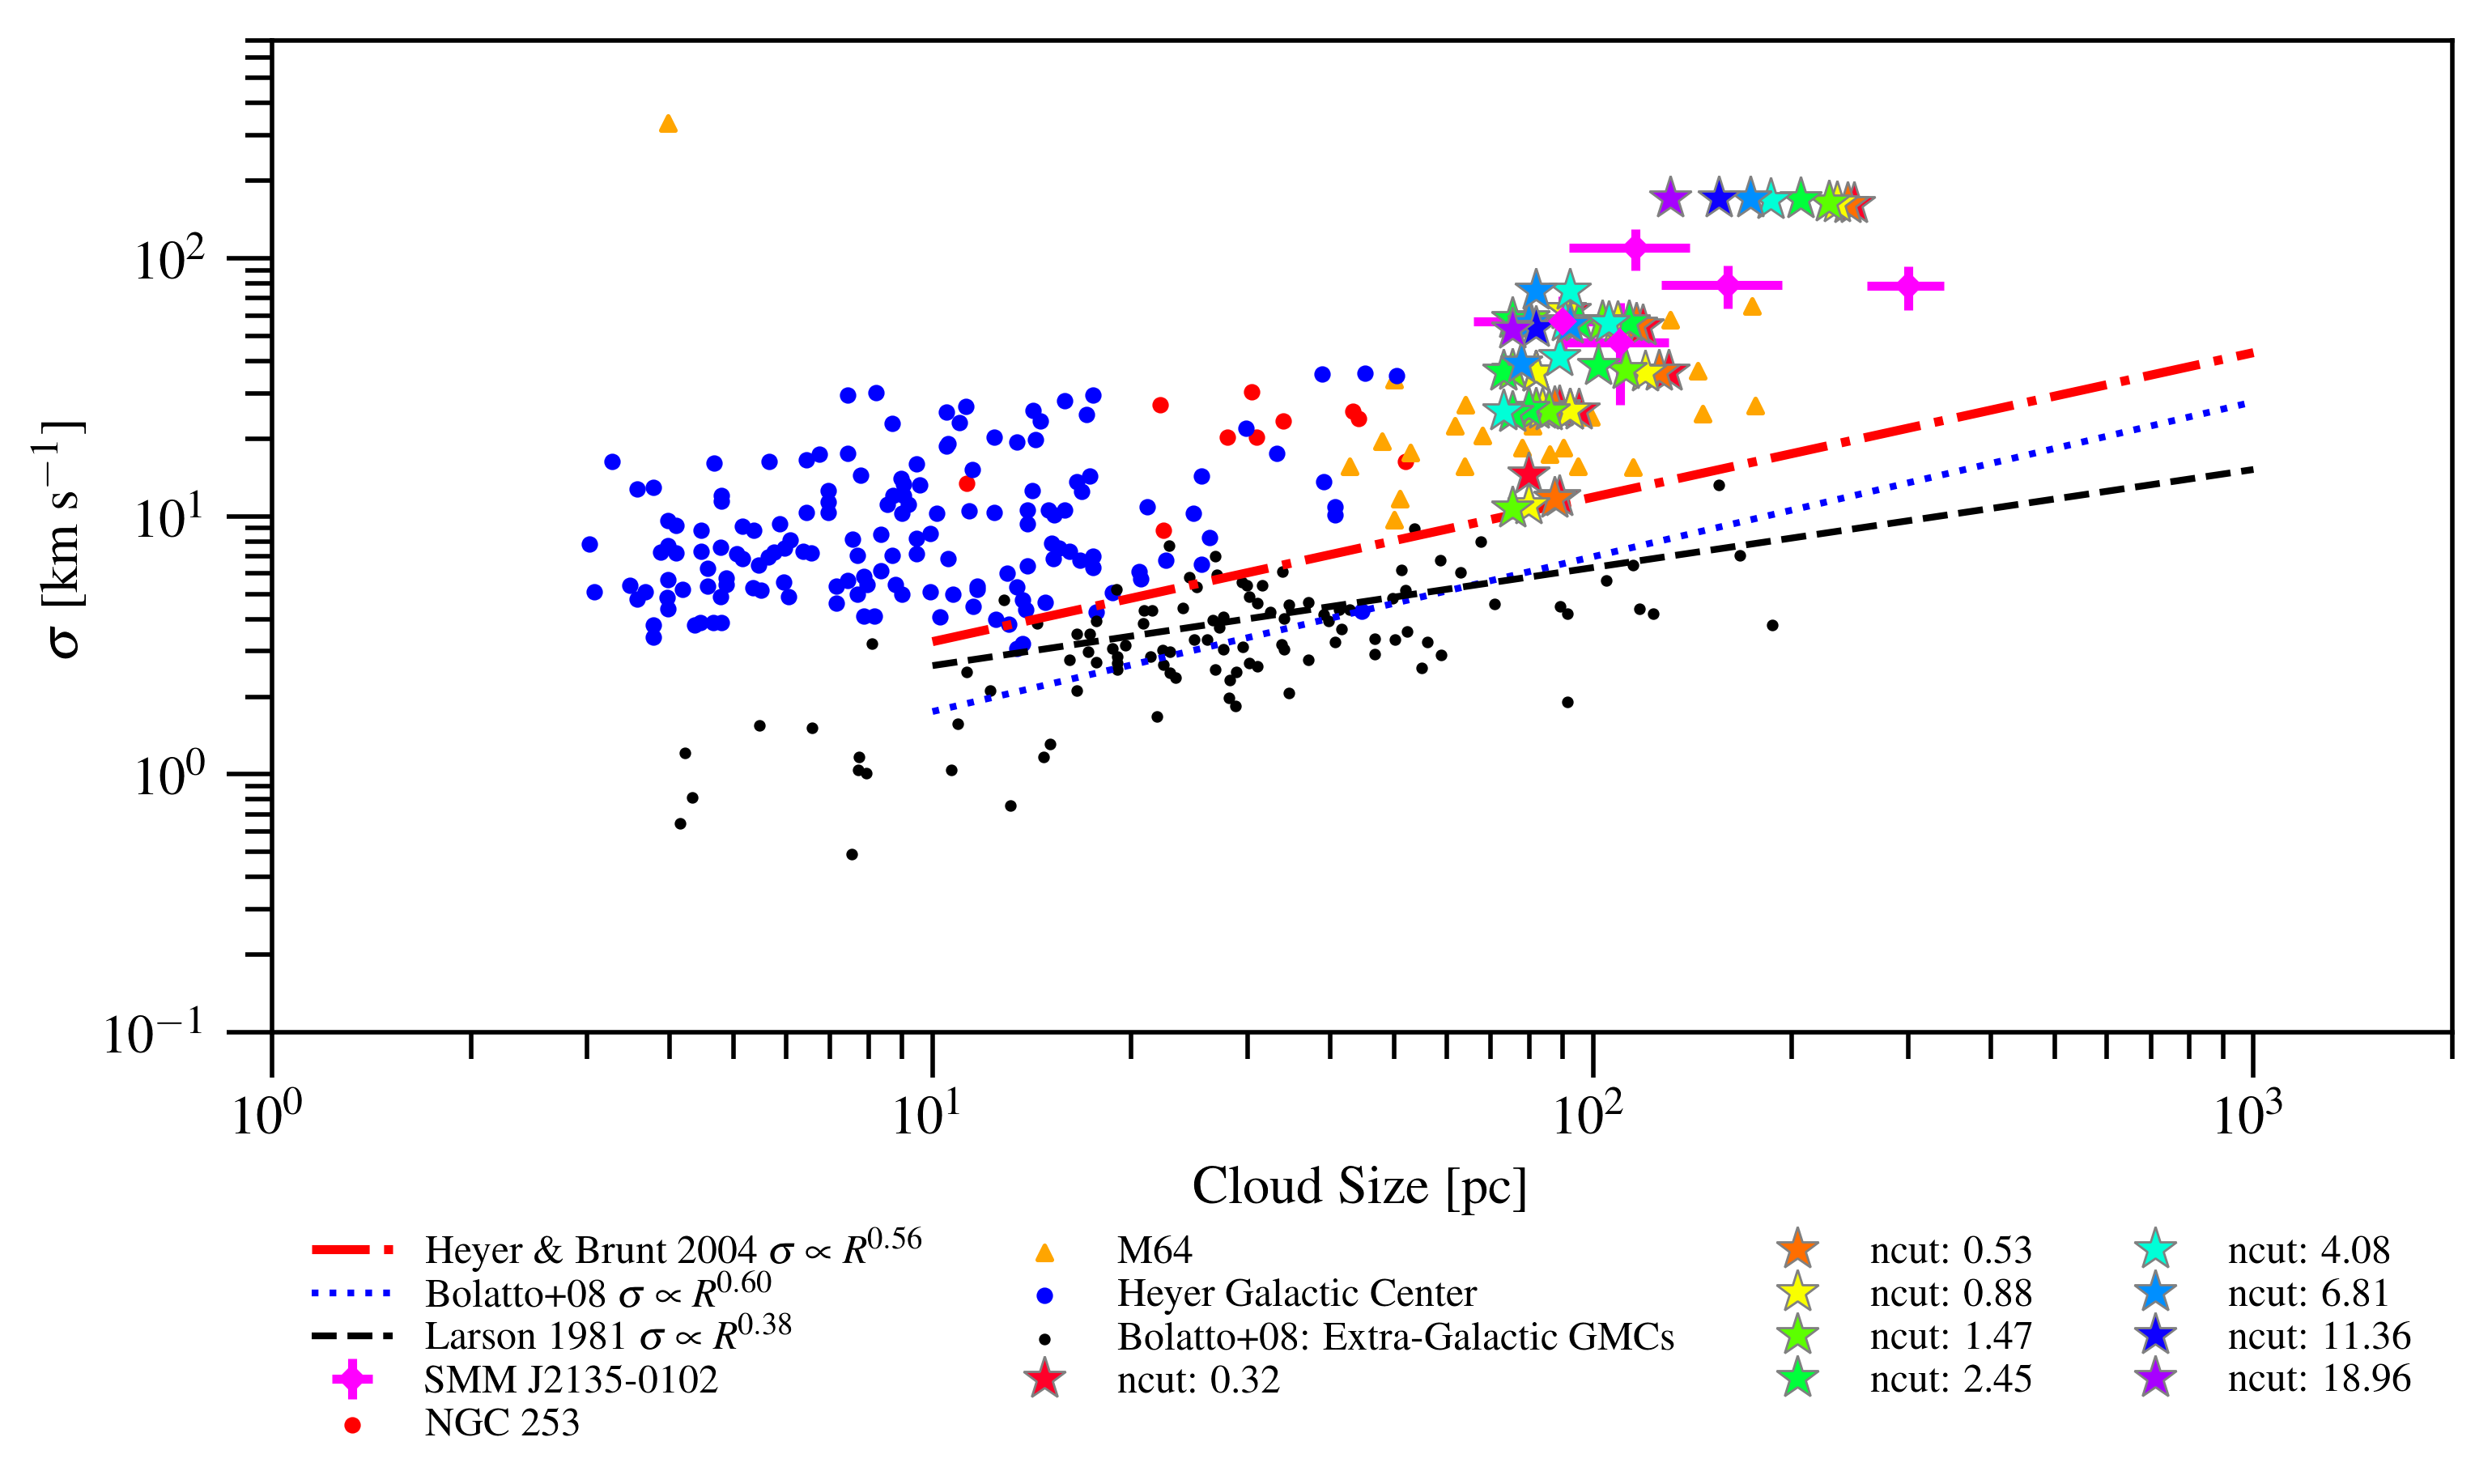
\includegraphics[trim=0 0 0 0, clip, width=0.85\textwidth]{\figpath/ss16_larsons.png}  
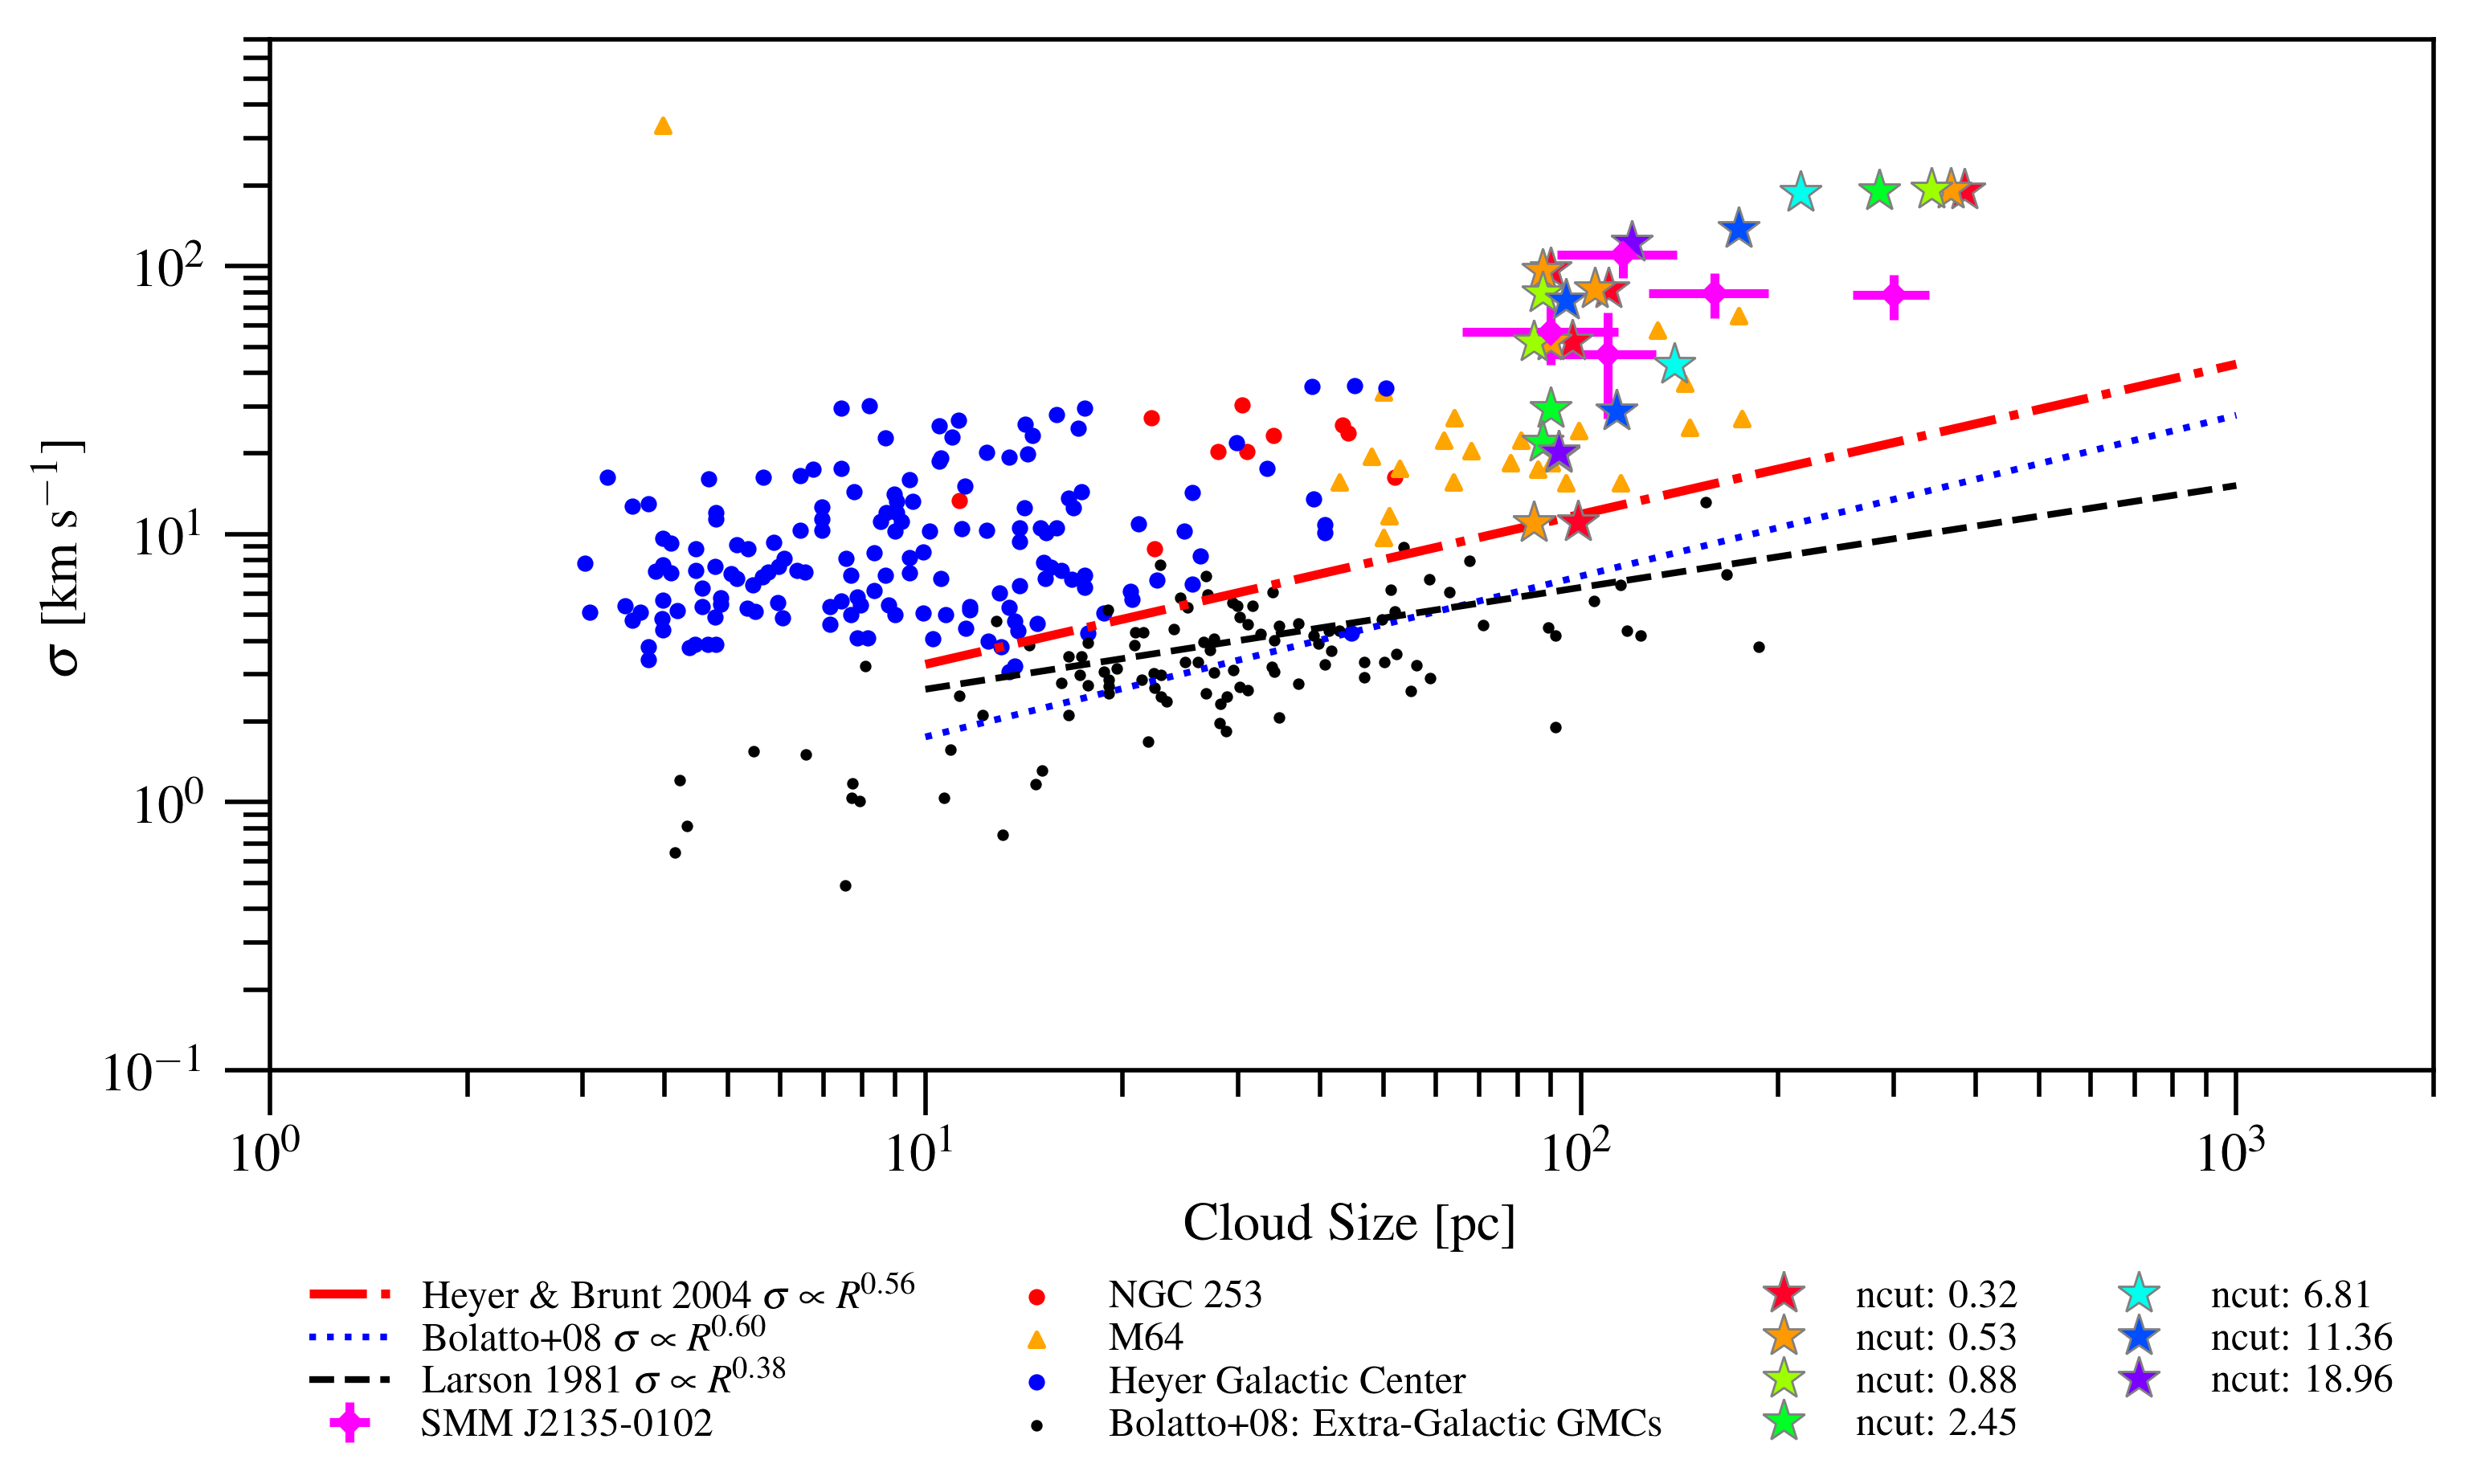
\includegraphics[trim=0 0 0 0, clip, width=0.85\textwidth]{\figpath/ss27_larsons.png}  
\caption{
Larson's relation of \flower in 
accreting phase (top) and
starburst phase(bottom) and 
those observed in nearby and the \z$\sim$2 star-forming galaxy.
\label{fig:larsons_single}}
\end{figure*}


\begin{figure*}[htbp]
\centering
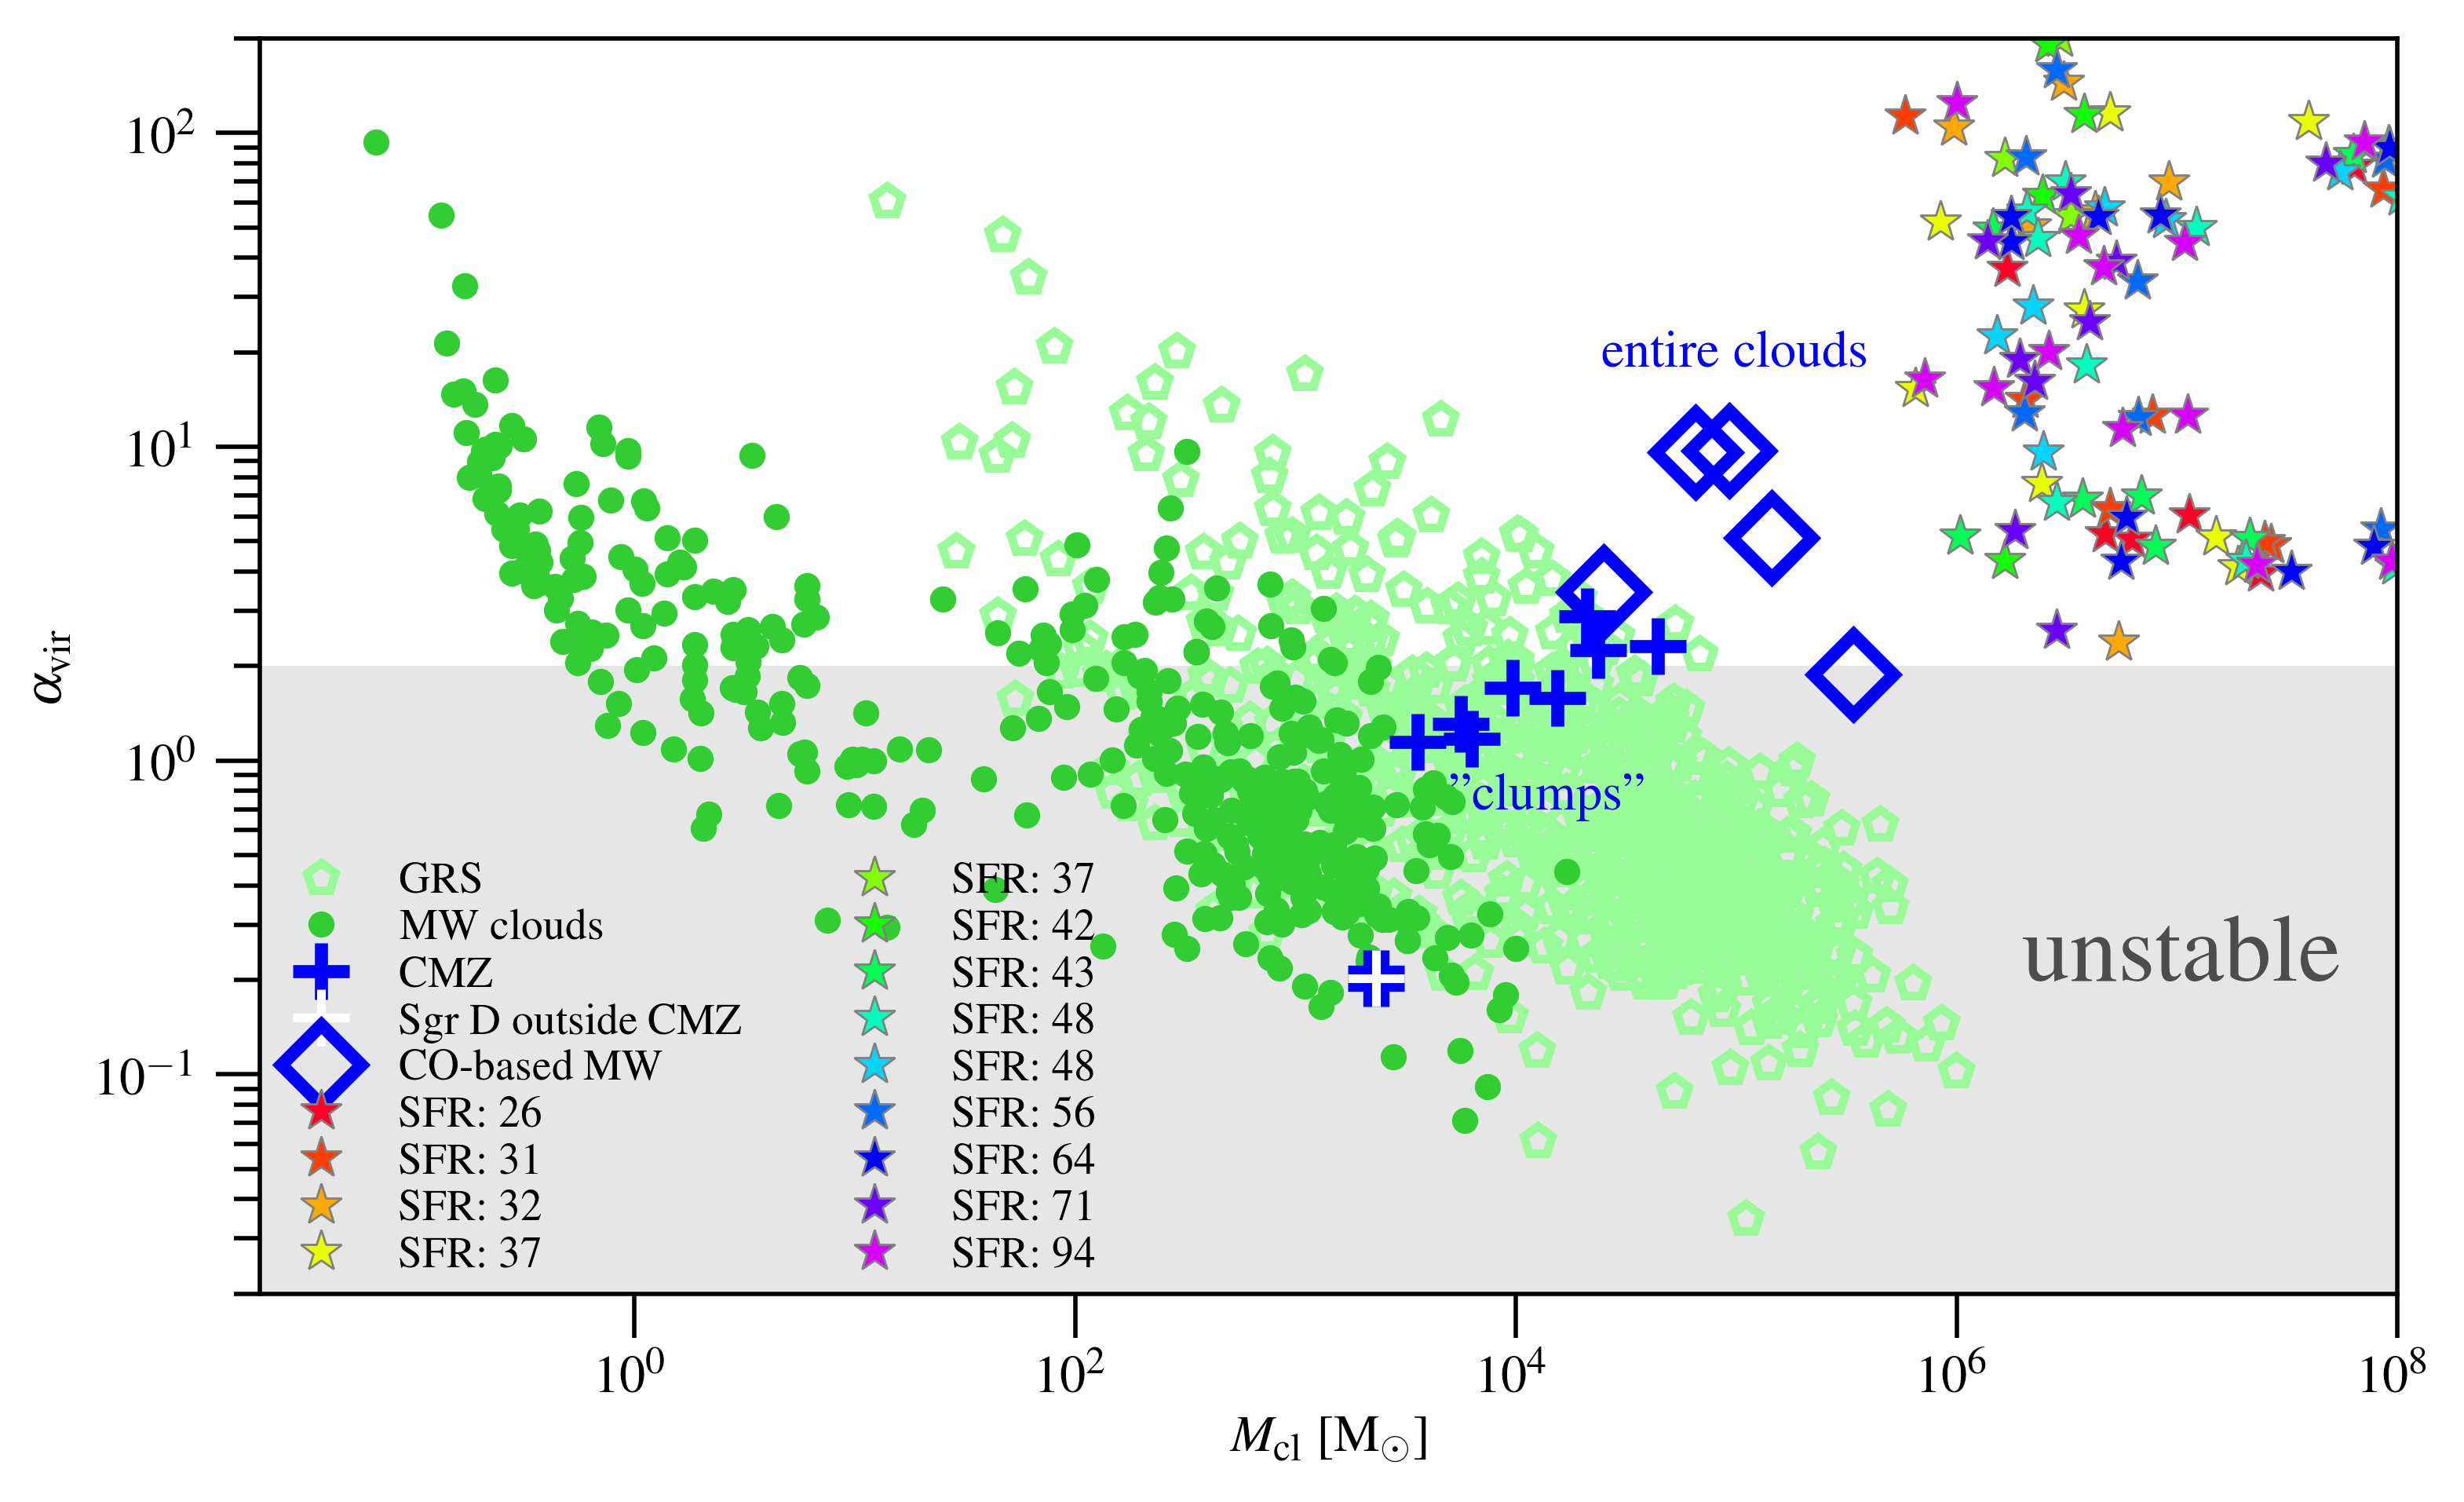
\includegraphics[trim=0 0 0 0, clip, width=0.85\textwidth]{\figpath/ss16-28_alphavir.png}  
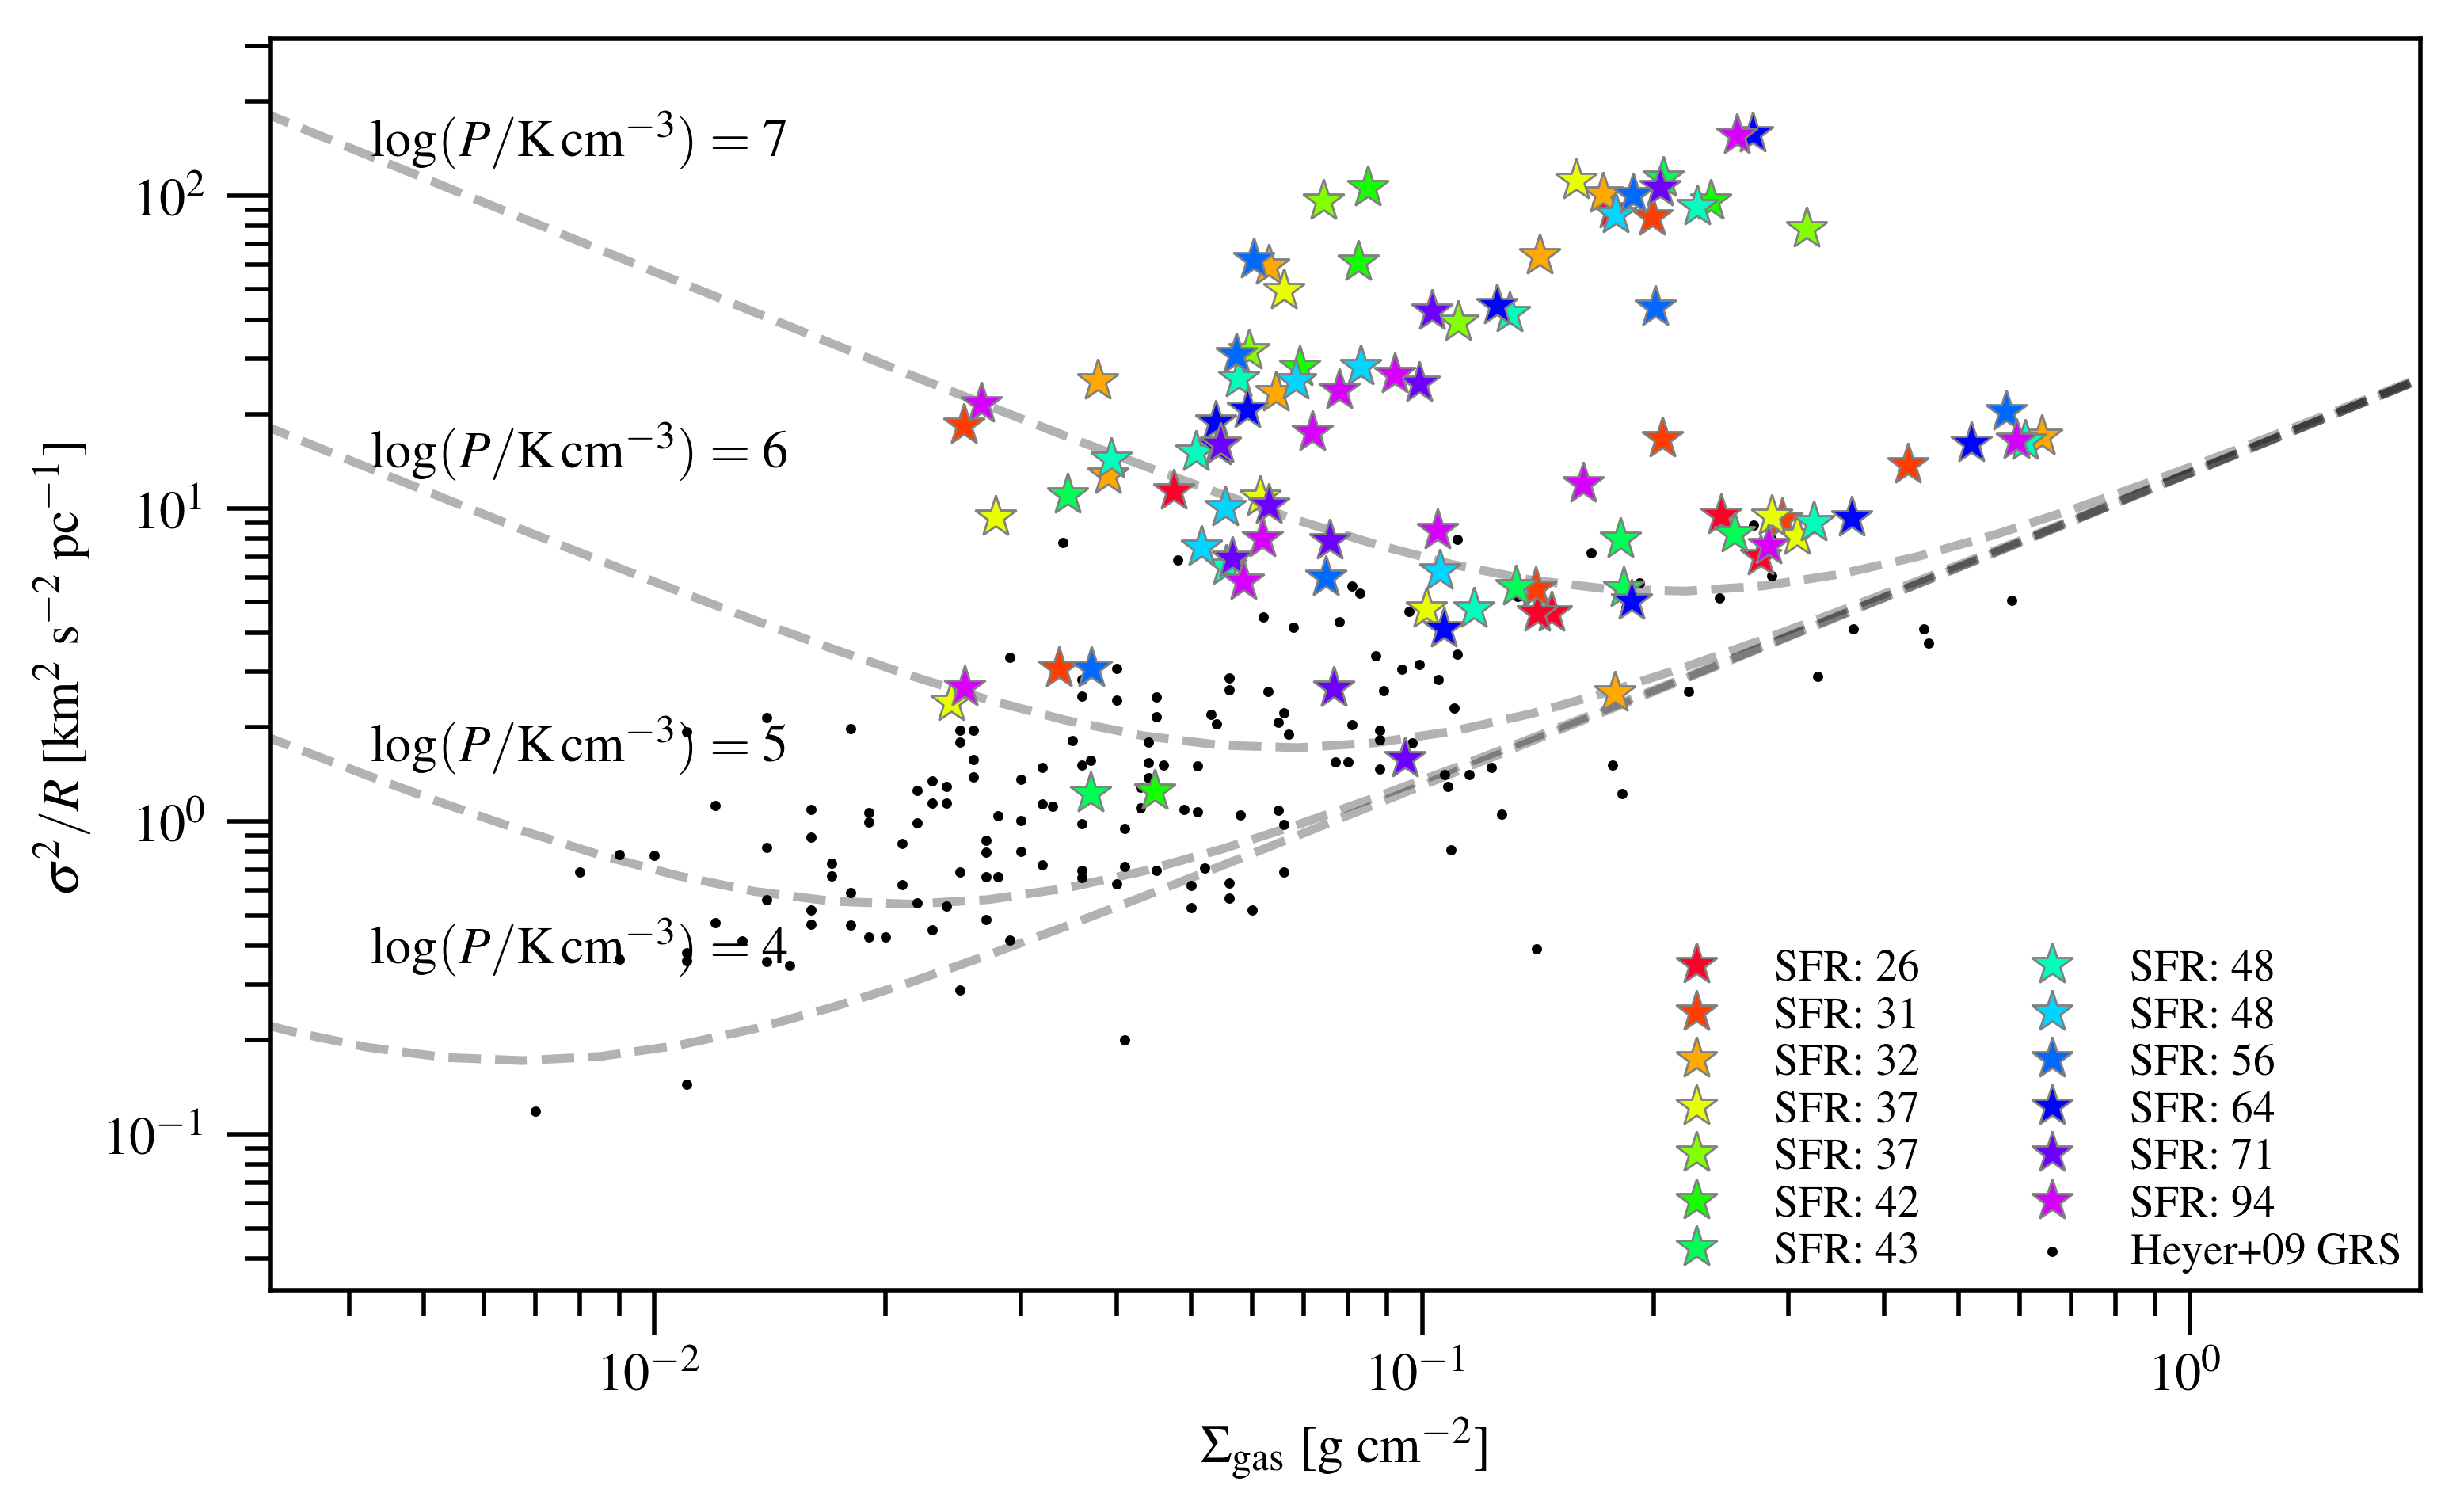
\includegraphics[trim=0 0 0 0, clip, width=0.85\textwidth]{\figpath/ss16-28_PVE.png}
\caption{
Top: Virial parameter and cloud mass of MCs in \flower identified across all snapshots.
Bottom: $\sigma^2/R - \Sigma_{\rm gas}$ relation of MCs.
\label{fig:alpha16-28}}
\end{figure*}

\begin{figure*}[htbp]
\centering
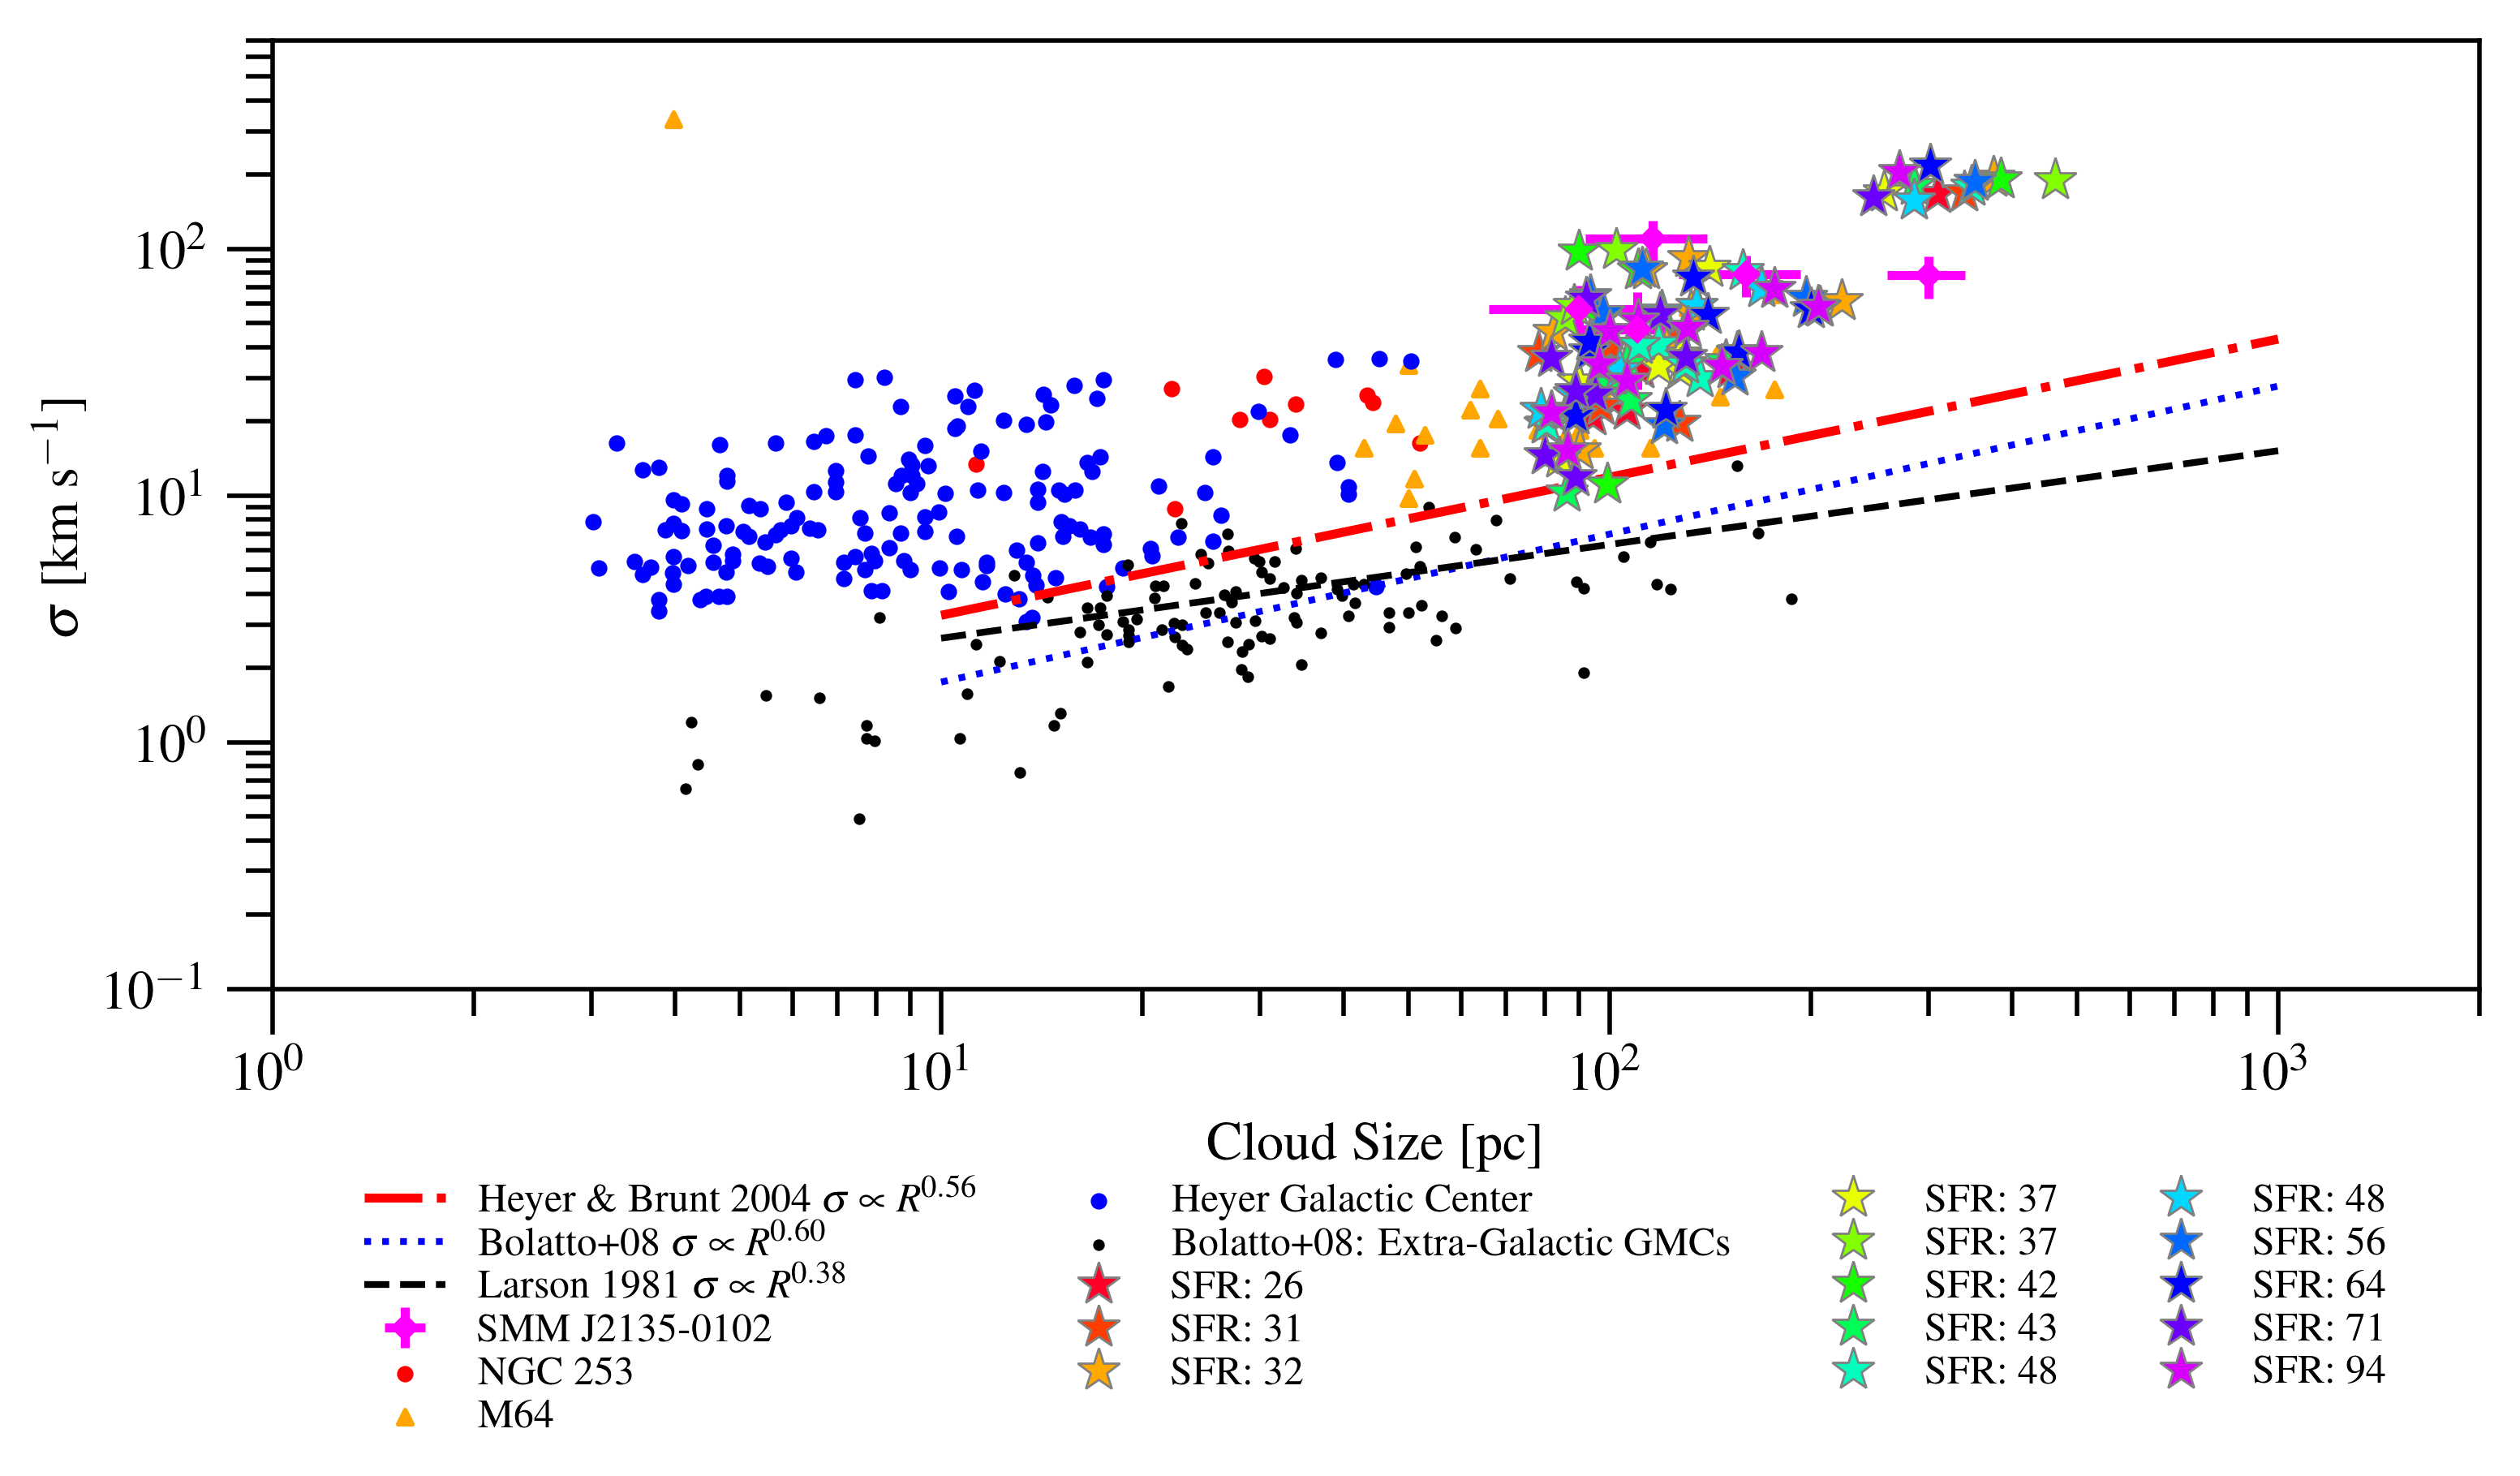
\includegraphics[trim=0 0 0 0, clip, width=0.85\textwidth]{\figpath/ss16-28_larsons.png}  
\caption{
Larson's relation of \flower across all snapshots (showing MC properties in different evolutionary 
phases) and 
those observed in nearby and the \z$\sim$2 star-forming galaxy.
\label{fig:larsons16-28}}
\end{figure*}


\begin{figure*}[htbp]
\centering
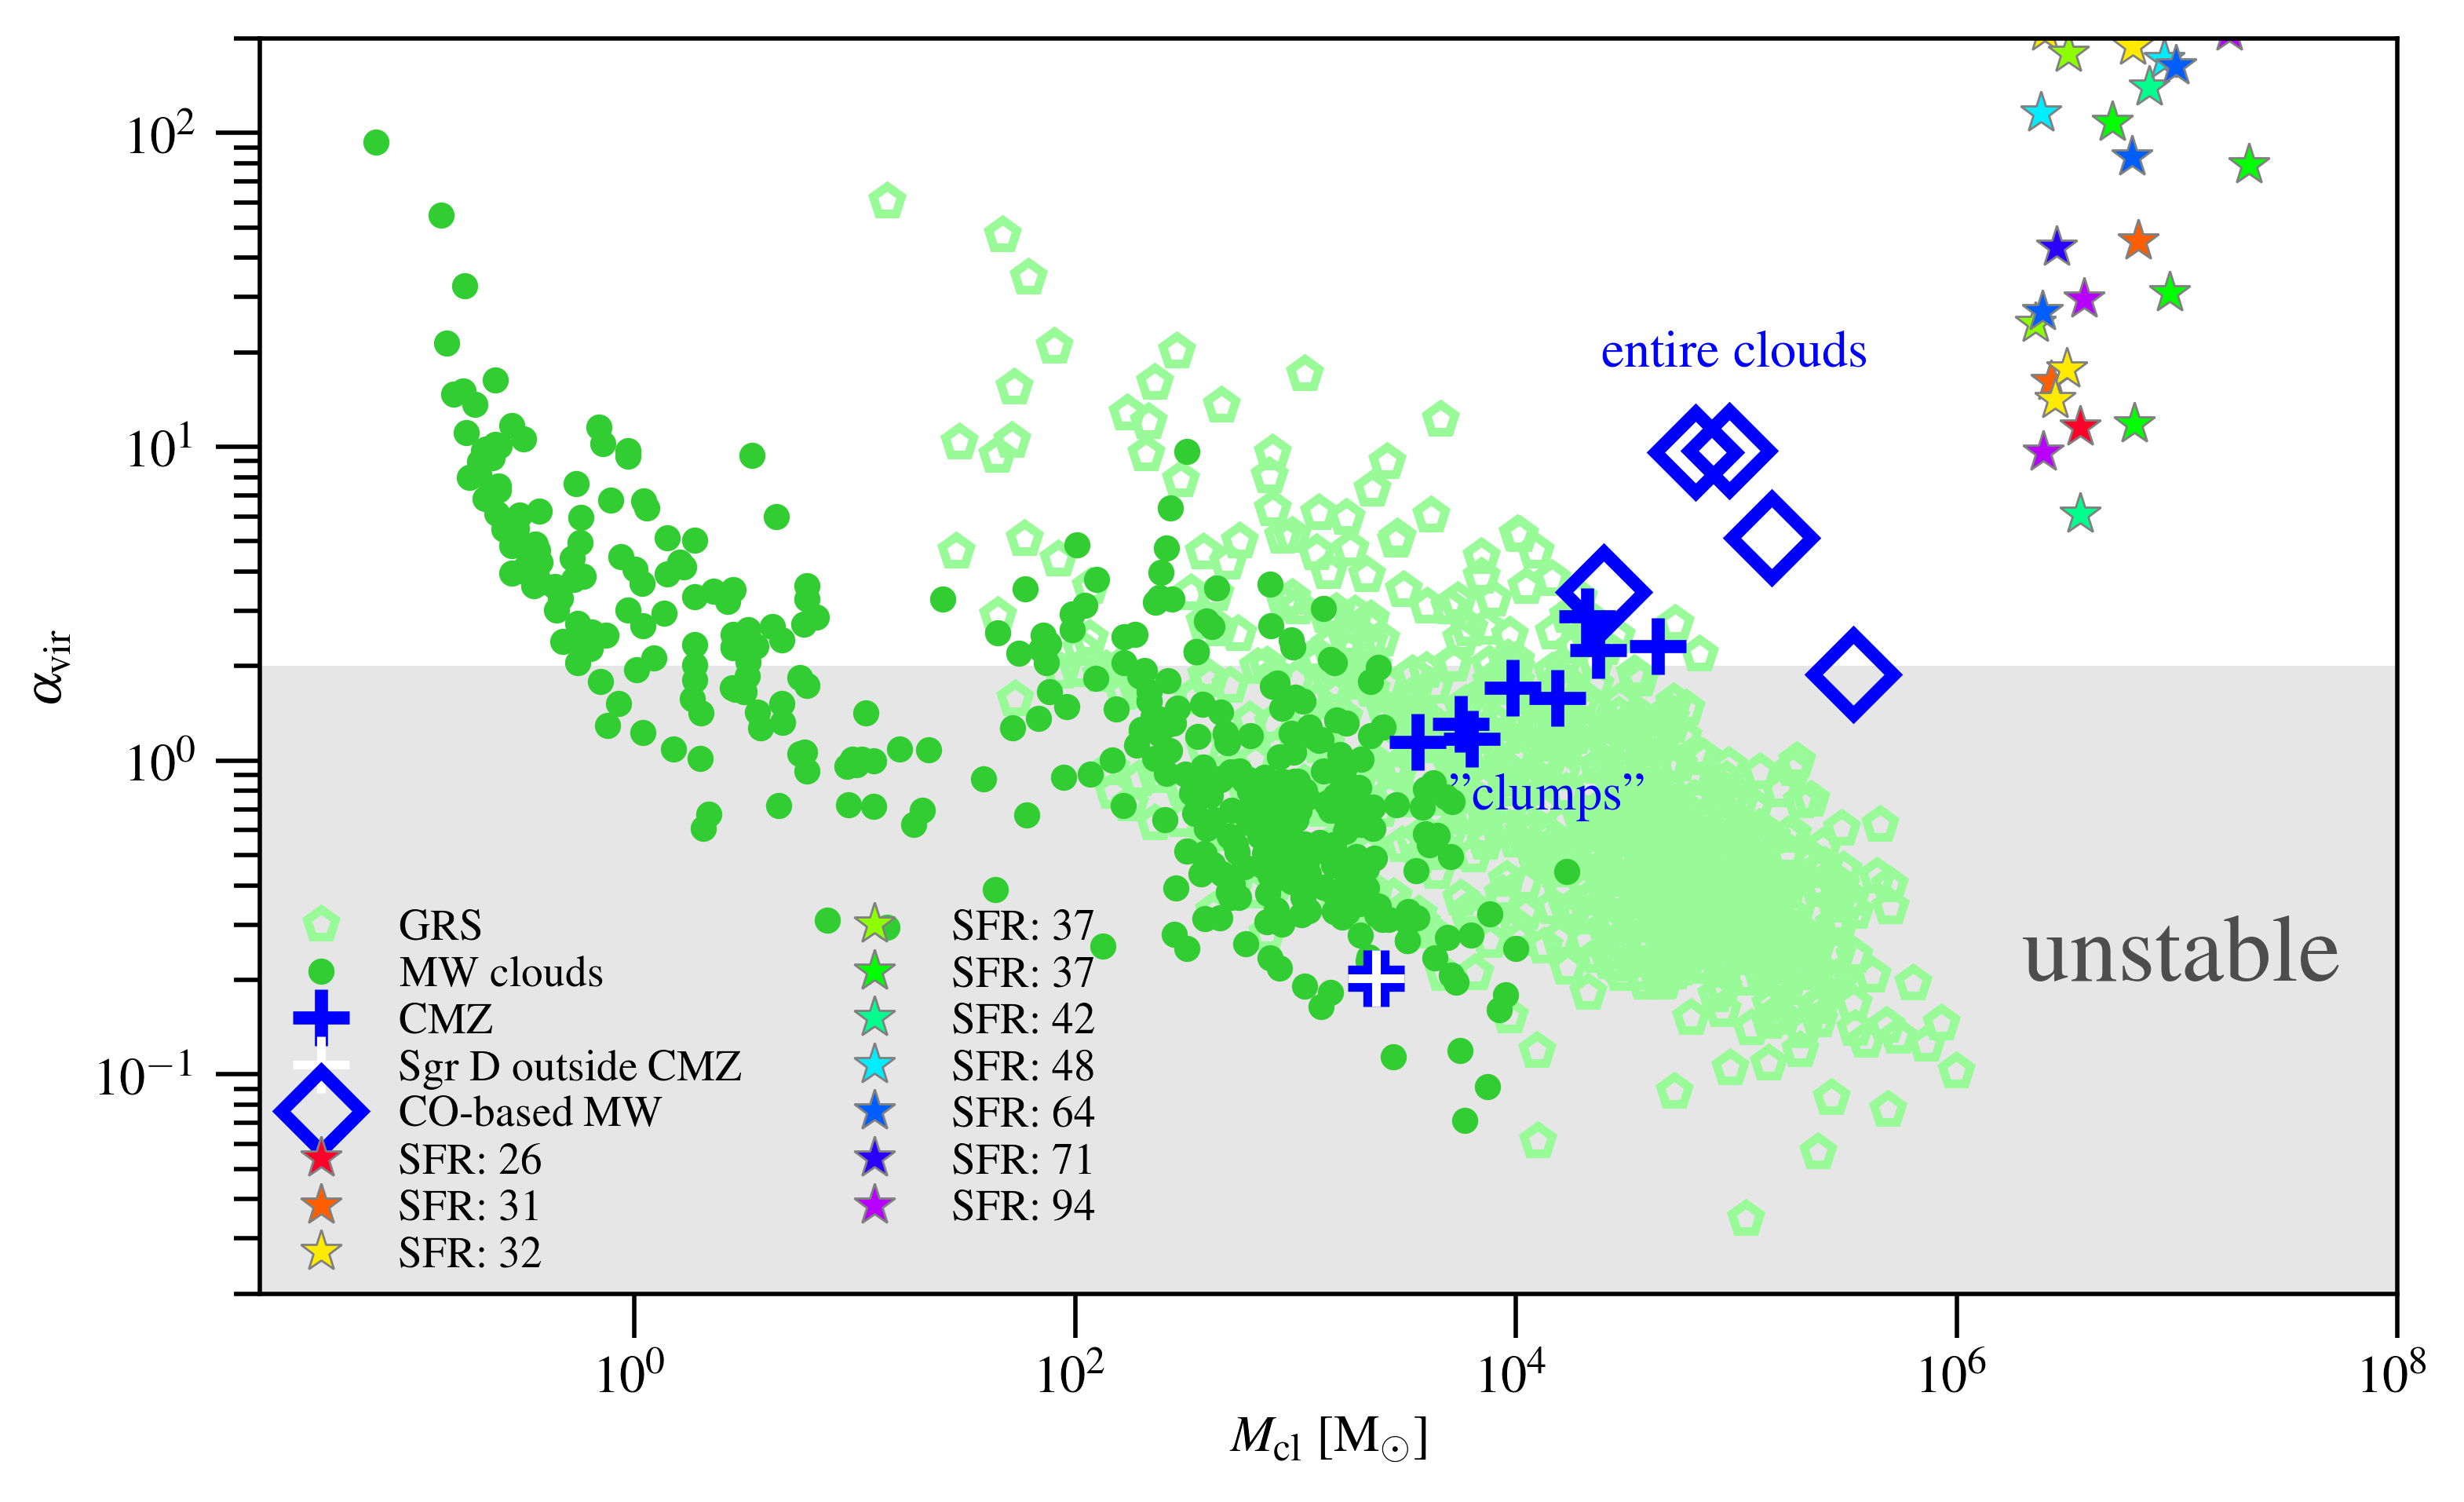
\includegraphics[trim=0 0 0 0, clip, width=0.85\textwidth]{\figpath/ss16-28-alphavir-highncut.png}
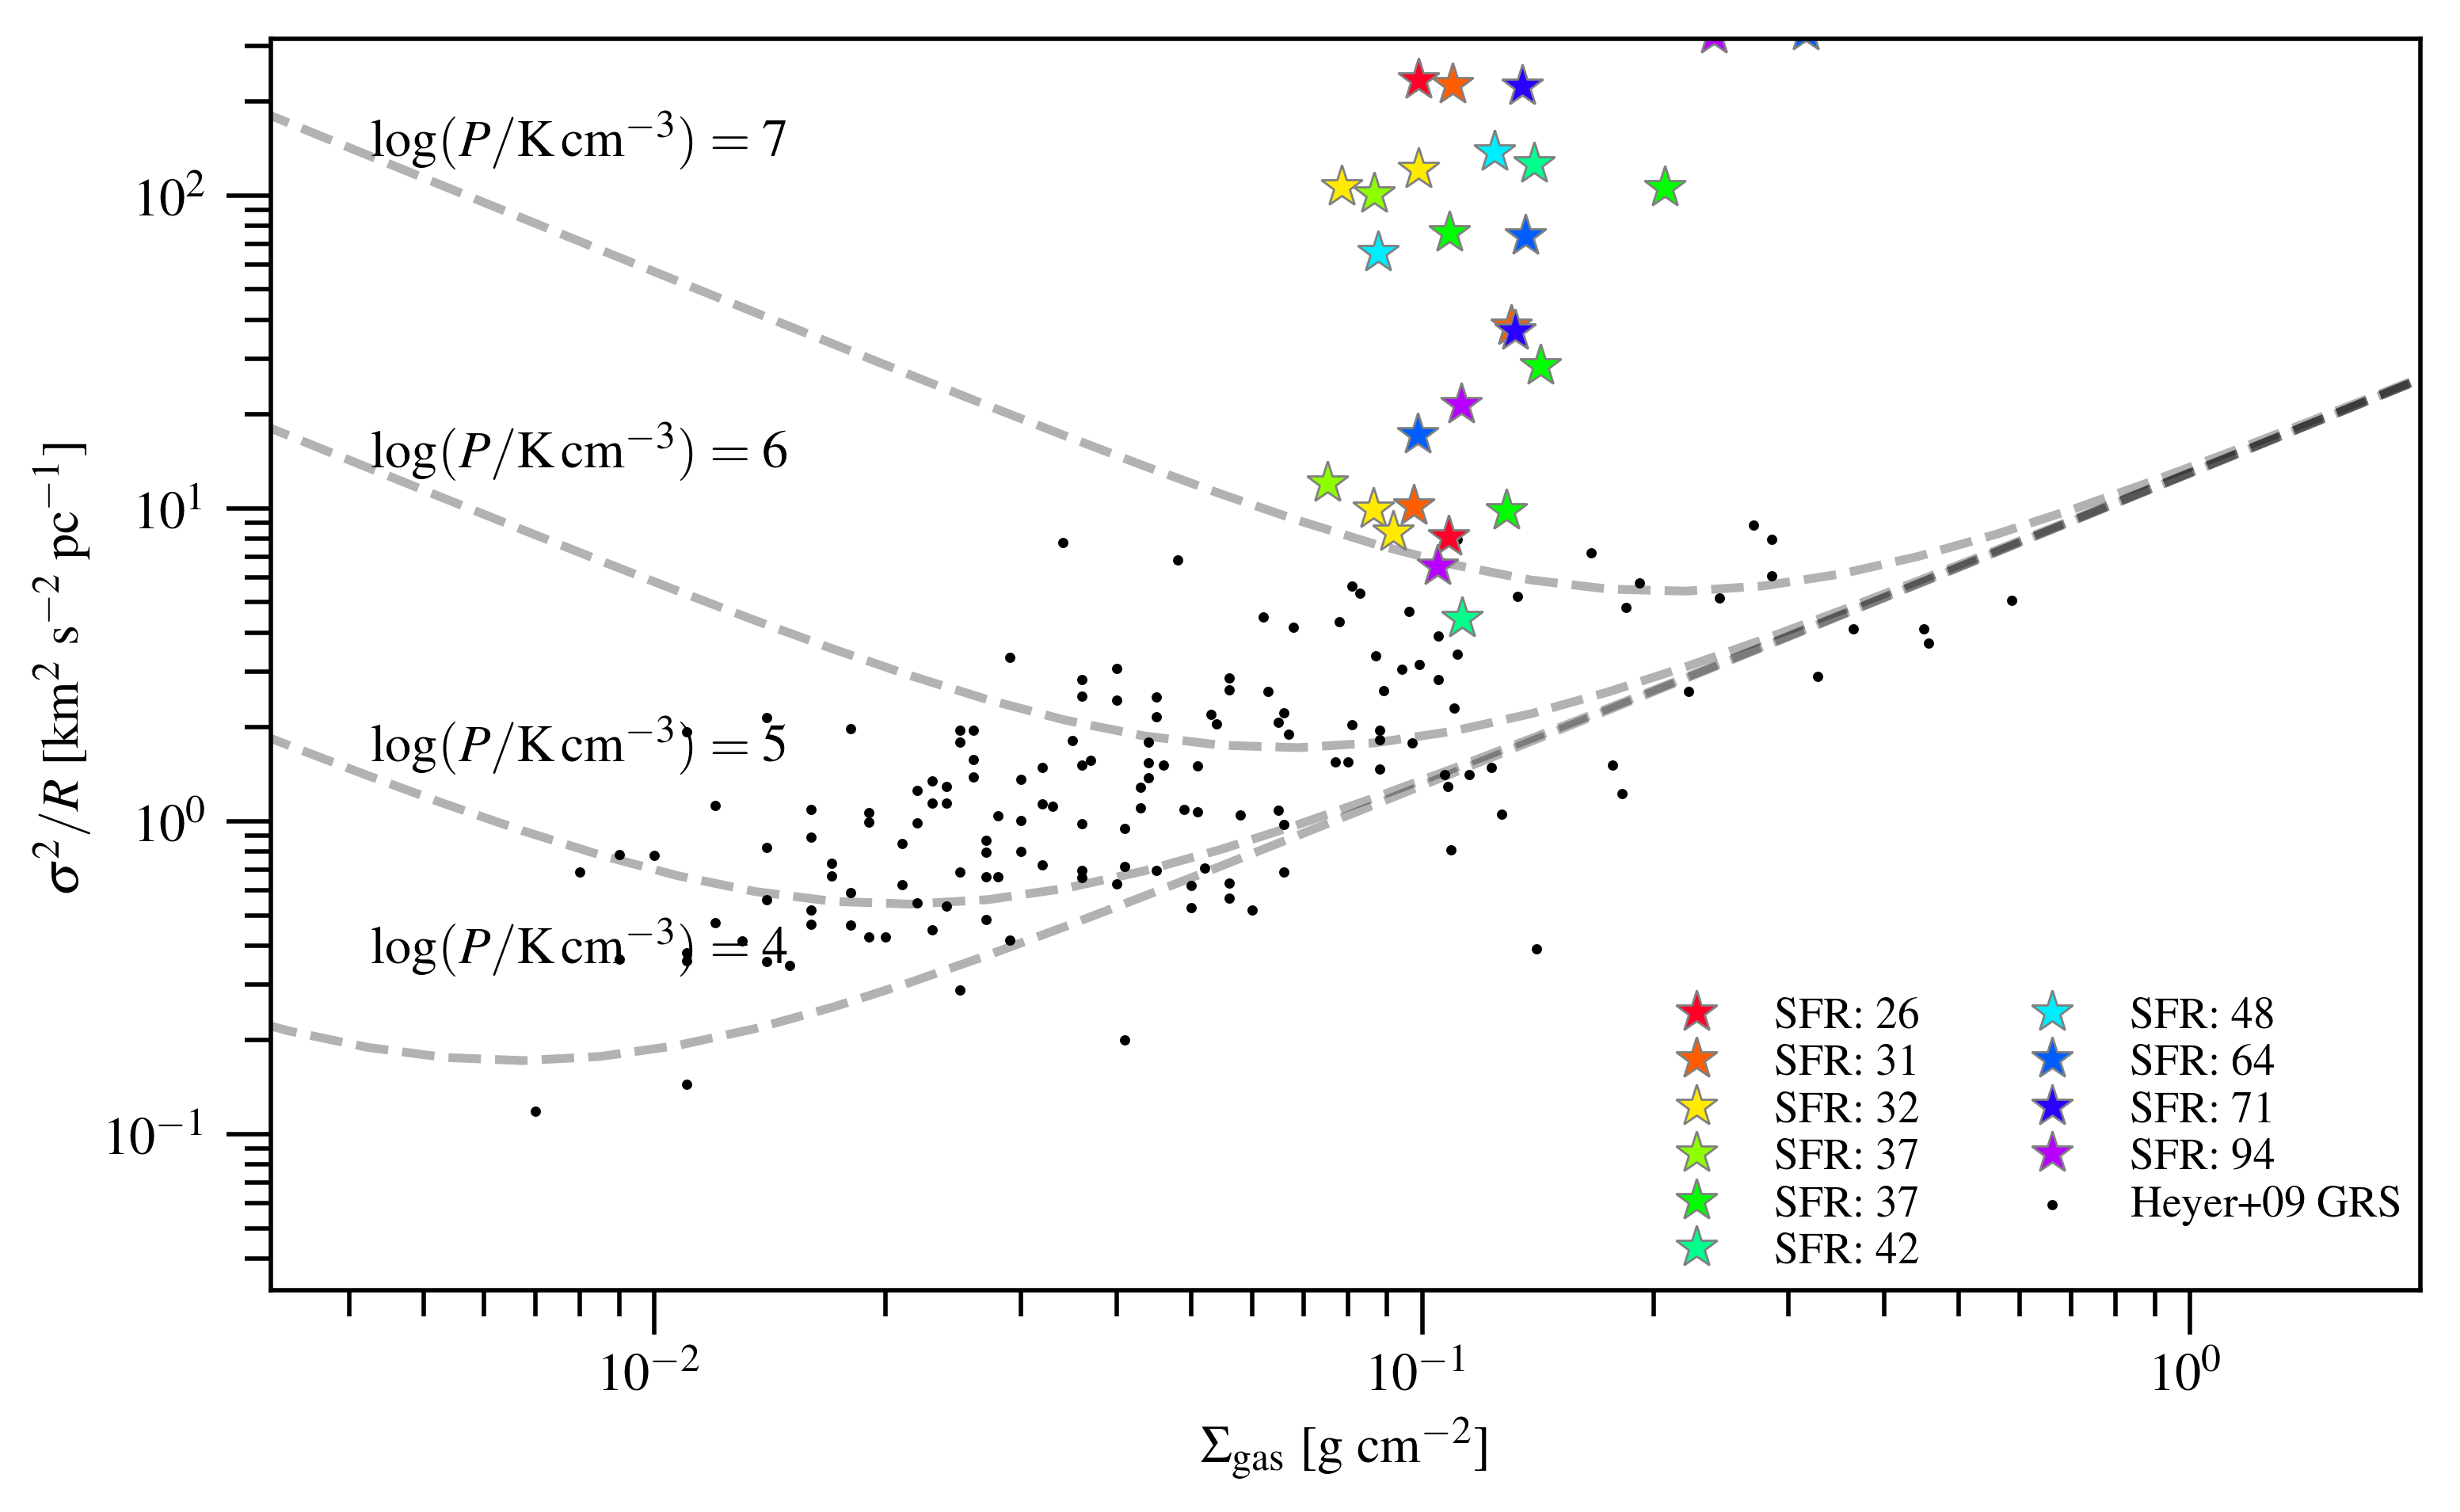
\includegraphics[trim=0 0 0 0, clip, width=0.85\textwidth]{\figpath/ss16-28-PVE-highncut.png}
\caption{
Same as \Fig{alpha16-28}, but MCs here are those identified from the highest $n_{\rm cut}$,
where only denser substructures of the main disk of \flower are included. 
\label{fig:alpha16-28-highncut}}
\end{figure*}

\begin{figure*}[htbp]
\centering
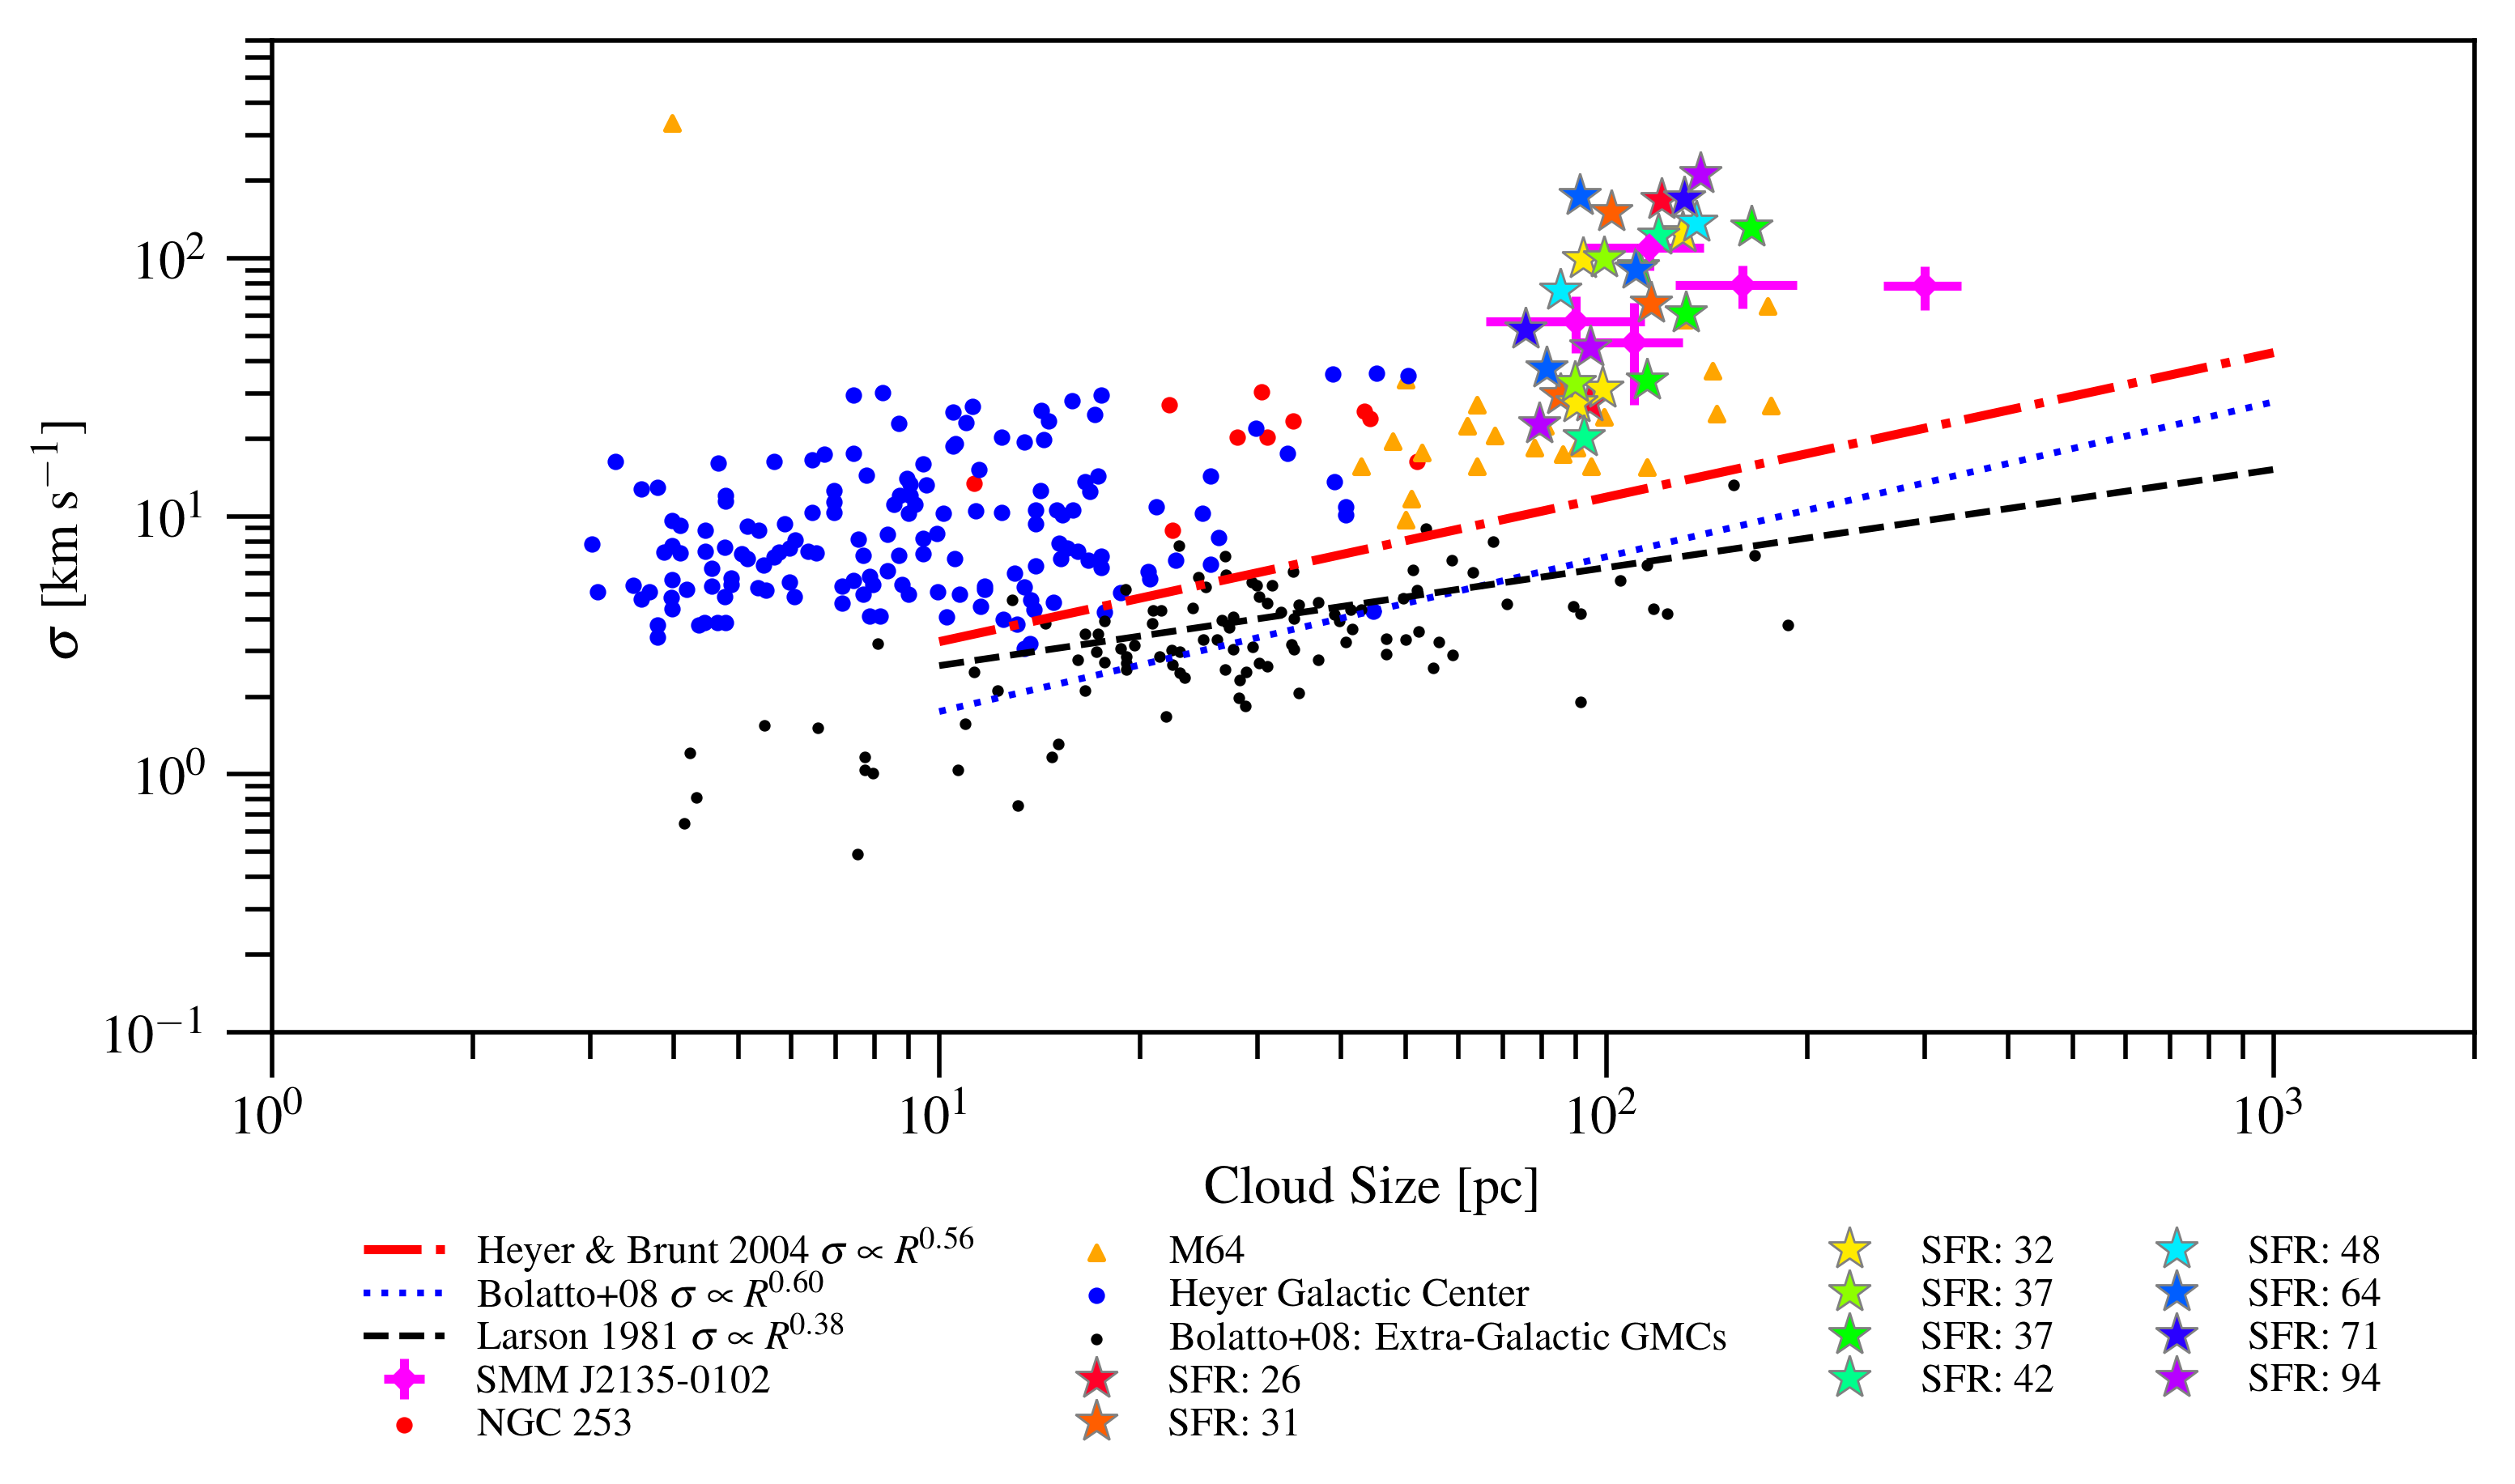
\includegraphics[trim=0 0 0 0, clip, width=0.85\textwidth]{\figpath/ss16-28-larsons-highncut.png}  
\caption{
Same as \Fig{larsons16-28}, but MCs here are those identified from the highest $n_{\rm cut}$,
where only denser substructures of the main disk of \flower are included. 
\label{fig:larsons16-28-highncut}}
\end{figure*}



\subsection{Variation in MC Properties Depending on Choice of Density Cuts}	 \label{sec:ncut}
% single Snapshot
We investigate possible variations in the dynamics of the molecular structures of \flower and its satellites 
to test 
the robustness of our results against the choice of density threshold in \Sec{ncut}.
That is, how sensitive are the structure properties, and thus, the conclusion of our study
dependent on the choice of density thresholds.
We vary the choice of H$_2$ density for each of the snapshots and 
find no obvious differences in our results (i.e., inferences on the dynamics of \z$\sim$\,6 
MCs in relation to those observed in nearby and \z$\sim$2 galaxies in the context of 
cloud scaling relations).
We interpret this lack of variation a manifestation of ..., and that, at least on the scales studied here, the cloud properties are what we found ... 
Our results is therefore robust, haha.

%\begin{figure*}[tbph]
% \centering
%\includegraphics[width=\textwidth]{\figpath/.pdf}  
%\caption{\label{fig:}}
%\end{figure*}



\subsection{Schmidt-Kennicutt Relation}
As benchmarking, we check the SK relation using the SFR and gas surface densities of the clouds. {\bf remind Pallo to look into this}.


\subsection{SFR-Mach Relation}
In \Fig{}, we show the relation between SFR and the Mach number ($\mathcal{M}$) for the molecular 
complexes identified. 
We find a positive correlation between the two quantities, with a Pearson-$R$ coefficient of xxx, 
which is unsurprising given that our simulations include the effect of stellar feedback. That is, 
the high $\mathcal{M}$ can be interpreted as a result of \SF resulting from feedback from 
massive stars.


\subsection{Clump Mass Function}

\begin{figure*}[htbp]
\centering
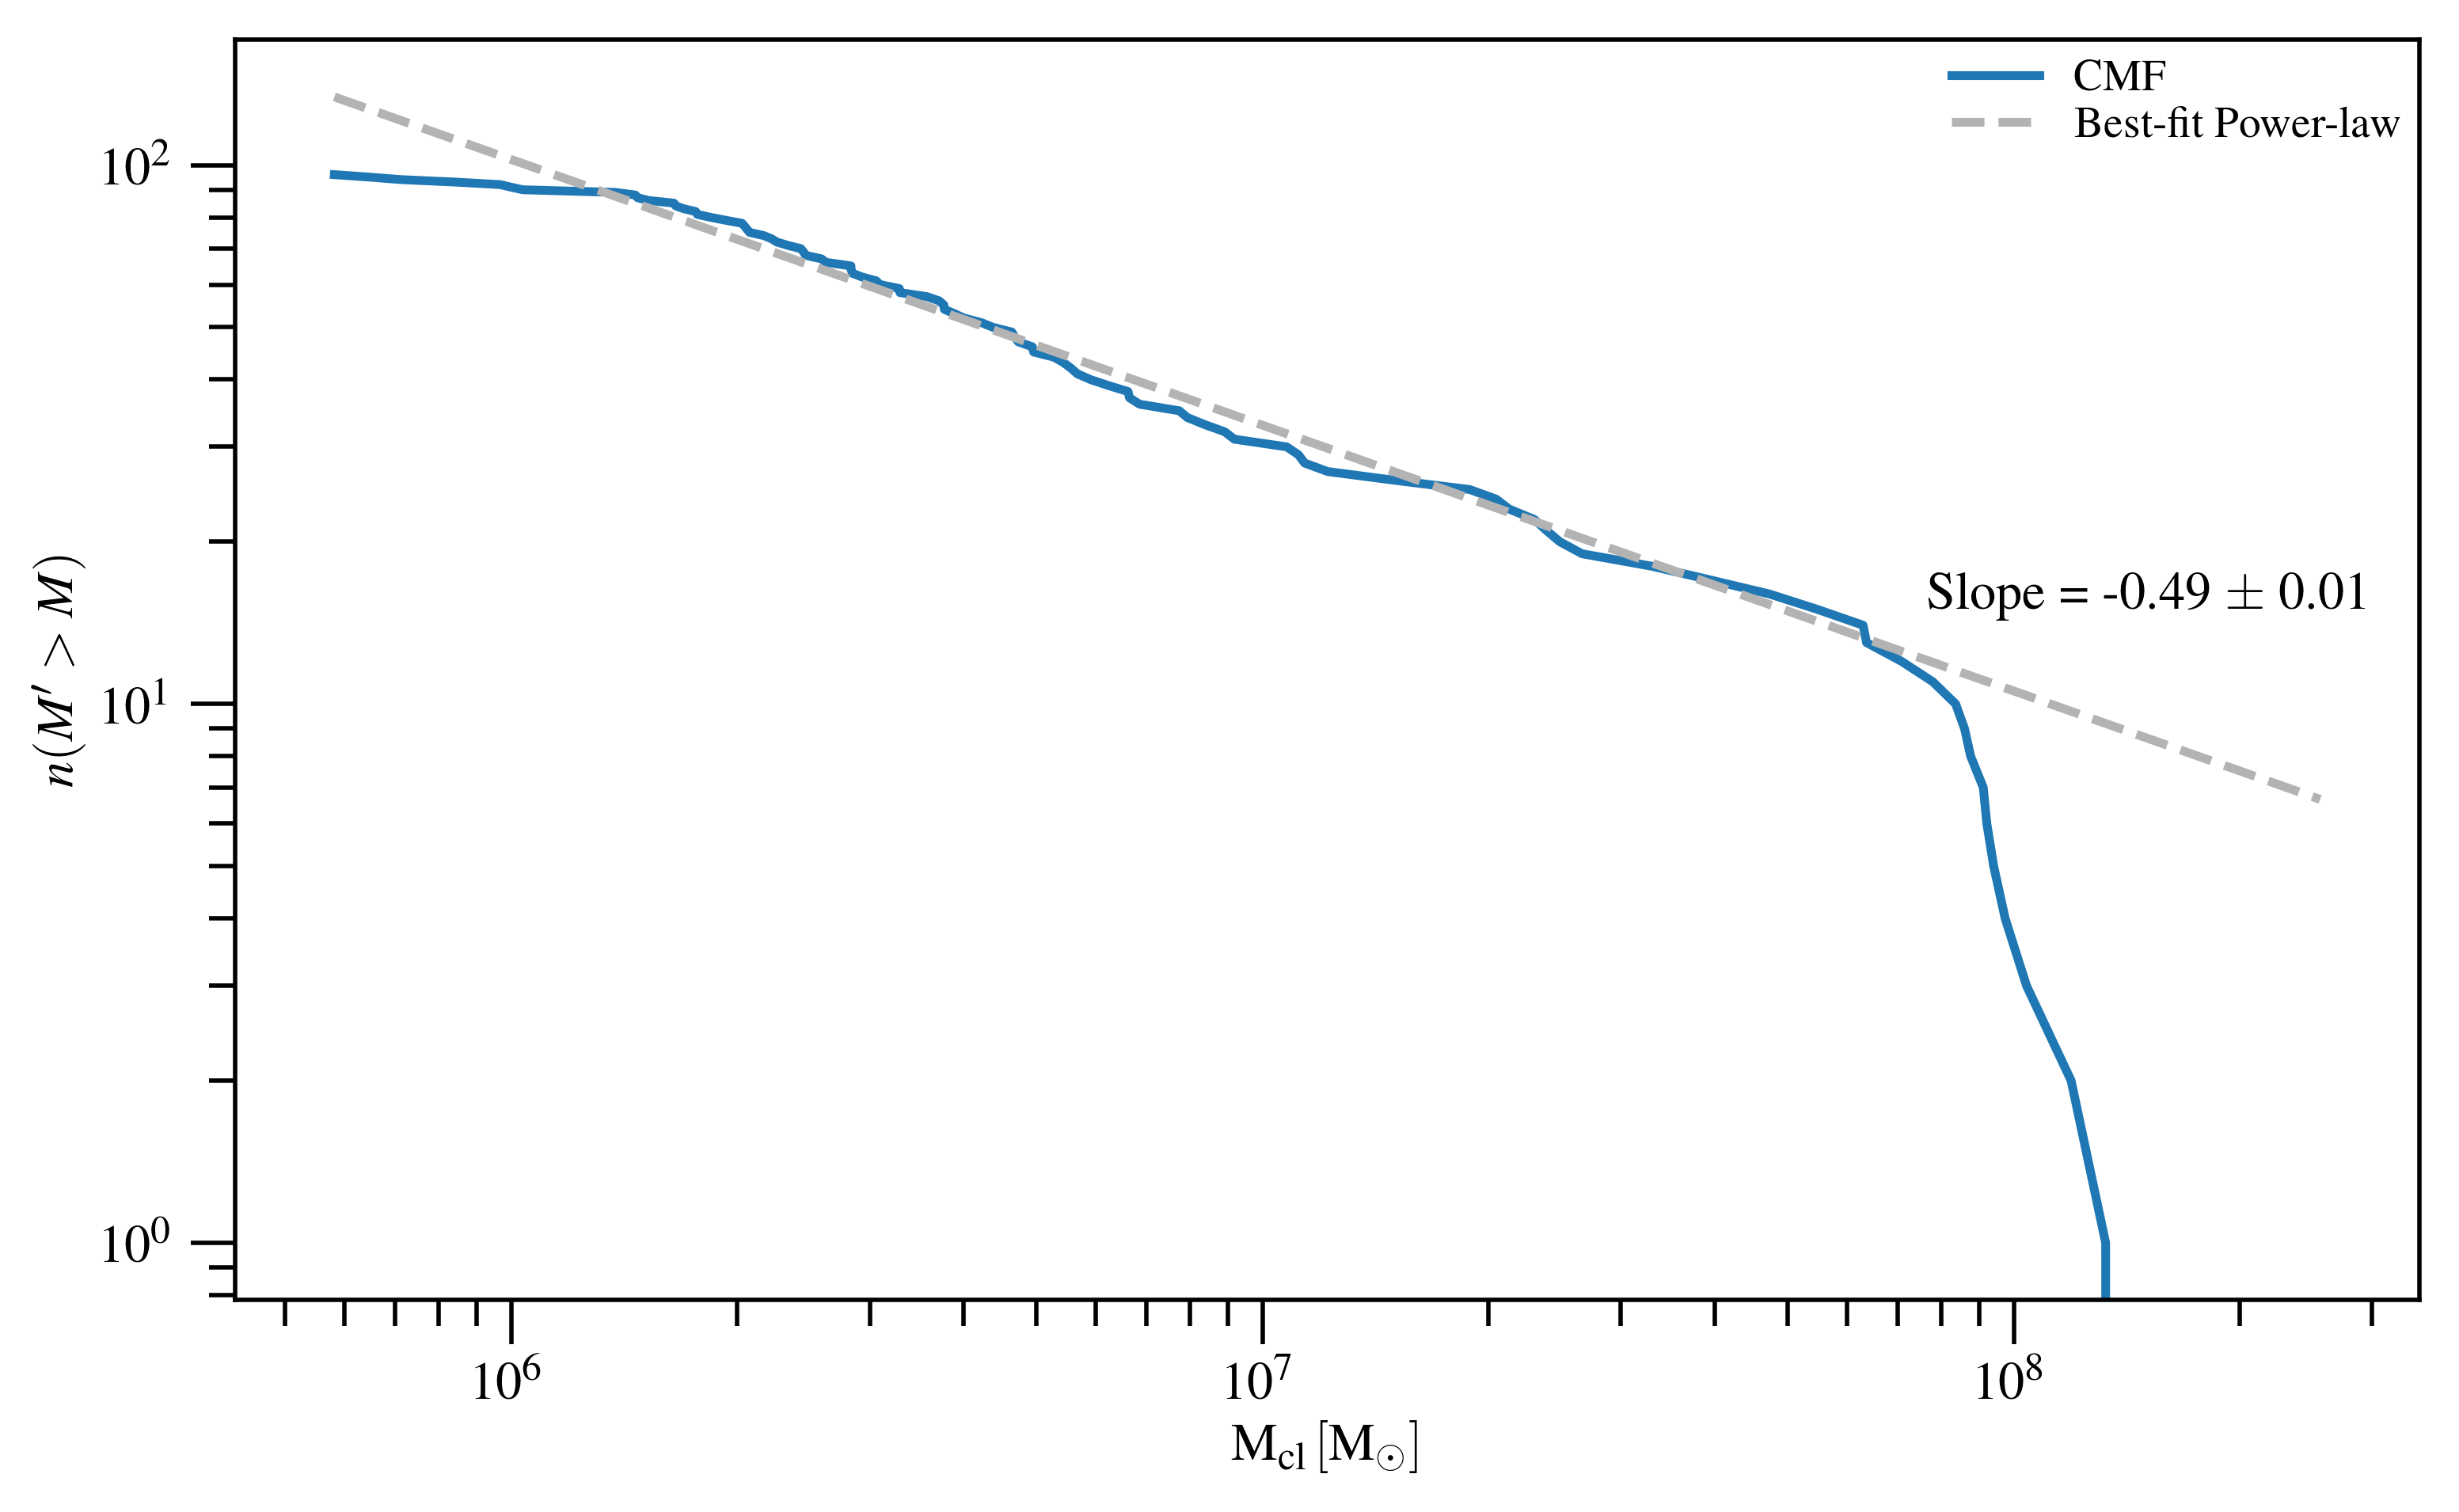
\includegraphics[trim=0 0 0 0, clip, width=0.85\textwidth]{\figpath/CMF_.png}  
\caption{
CMF of MCs in \flower and best-fit power law.
\label{fig:cmf}}
\end{figure*}

Noisy due to resolution effect, since we only have one galaxy here. However, 
we could improve the ``signal-to-noise'' ratio by including clouds identified from different 
snapshots (valid unless in some snapshots, the galaxy experience a violent event).
We find a shallower slope in the CMF of \flower (\Fig{cmf}) 
compared to those observed in nearby galaxies (based on a sample of 
$\sim$70 resolved GMCs in M31, M33, IC10 and the Magellanic Clouds; \citealt{Blitz07a}).

While our result, of particular relevance here is the slope of the CMF, is subject 
to the uncertainties in the analysis method and the resolution of our simulation --- i.e., that is 
we are likely biased to finding more massive clouds.
High resolution simulations will be useful to shed light on 
the evolving dynamical properties of the lower-mass molecular structures in 
galaxies at EoR; however, they are more expensive to run.
On the contrary, an advantage of using cosmological zoom-in simulations for this study
is that our computational boxes are not closed, allowing us to examine how 
the molecular complexes' properties vary under the influence of gas inflow/outflow.


\section{Mass Scales set by Toomre and Jeans Instabilities}

In the limit of a thin rotating disk, rotation can help stabilizes self-gravitational contraction for wavelengths greater than the Toomre length:
\begin{equation}
\lambda_T = 4\pi^2 G\Sigma/\kappa^2,
\end{equation} 
where $\kappa$ is the epicyclic frequency (\citealt{Toomre64a}).
However, if the condition $Q<Q_{\rm crit}$ is satisfied, where the latter is set by 
the thermal pressure, then fragmentation can happen 
(e.g., instability impose by angular momentum from gas accretion from the cosmic web and 
satellite galaxies and stellar feedback).



%--------------------------------------------------------------------------
%                                Discussion
%--------------------------------------------------------------------------
\section{Discussions and Implications}     \label{sec:diss}
Yet.... at the epoch of reionization.... For instance, to resolve the 
\aco line emission in a $L^*$ prototypical galaxy at \z$\sim$6 on xxx\,pc 
require .... on-source time even with ALMA. 

Connection to observations

The largest molecular structure identified is essentially the main disk of \flower, which is ``broken'' down into smaller 
spatial and mass structures that are also denser as we increase $n_{\rm cut}$. In any case,
the MCs we identified are much bigger in size and mass than nearby GMCs, which is consistent with 
those observed in \z$\sim$2\,$-$\,4 galaxies with spatially resolved \obs.

Looking at correlations between physical parameters such as xx, yy, zz and the CMF 
can provide valuable information for developing models of \SF at EoR and 
galaxy evolution.


\subsection{Virial Parameter}
We quantify how stable a molecular structure is using the virial parameter, which 
describes the balance between pressure support and gravity. 

The high $\alpha_{\rm vir}$ suggest that the majority of the MCs identified are not collapsing. 
The largest structures are presumably supported by galactic rotation and turbulence from the feedback of 
multiple episodes of \SF.
Turbulence in the smaller denser clouds are expected to cascade down over a timescale of $\sim$xxx\,Myr, after which the cloud will collapse 
(its substructure likely collapses earlier than this timescale since turbulences would have dissipated). 

While it may appear that there is an inconsistency between the high $\alpha_{\rm vir}$ 
nature of the majority of the molecular gas in \flower and its SFR. 
That is, if most of the molecular gas in \flower has high $\alpha_{\rm vir}$, why does it sustain its high SFR of $\sim$100\,\Msun\,yr\pmOne?
This discrepancy can be explained in two ways. 
First, our results are limited by the resolution of the simulation, such that, in each MC, there 
likely exist multiple smaller-scales molecular structures (e.g., clumps and cores), 
as in the classical MC hierarchy. These smaller structures likely no longer supported by large-scale gravitational potential and differential rotation, 
and turbulence has dissipated rapidly on these scales to enable collapse \citep{Clark04a}.
Non-axisymmetric perturbations (e.g., arms) to the gravitational potential 
can induce orbit crossing, shocks and dissipation in gas, promoting turbulence dissipation.
Note also that \citet{Pettitt18a} report that the virial parameter could be a poor indicator 
for the star-forming capacity of the massive (10$^{5-6}$\,\Msun) ``clouds'' in their simulation. They 
do not find any significant correlation between $\alpha_{\rm vir}$ and cloud mass 
and the star formation efficiency ($M_*/M_{\rm cl}$).



\subsection{Larson's Relation}
The Larson's relation... empirically-motivated.


\subsection{CMF and IMF at EoR}



While first stars and galaxies are cooled predominated via H$_2$ lines. 
As shown in the $T-n$ phase plot in Fig. 8 of \citealt{Pallottini17b}, metals also play an important role in the cooling of early galaxies.


CMF influences the IMF because .. different cooling properties will lead to different xxx, and thus, Jeans mass/thus determines the final properties of the cloud fragmentation....  For instance, massive protostellar clumps are always supersonic, thus their internal structure are complex. They may form multiple stars.


The minimum clump mass M$_{\rm min}$ is limited by numerical resolution of our simulation. We do not have a resolution study (in hand) and so we cannot quantitatively evaluate this at the moment. The minimum clump mass allowed 
by our clump finding algorithm is the mass over 10 cells that exceeds the given threshold density.



%--------------------------------------------------------------------------
%                                Conclusions
%--------------------------------------------------------------------------
\section{Summary and Conclusions}      \label{sec:conclusion}

We study the dynamical properties of molecular complexes in a \z$\sim$6 lyman-break galaxy, 
at the end of the epoch of reionization, using state-of-the-art cosmological zoom-in simulation 
(\ncode{Serra}). We identify molecular cloud complexes in the main galaxy of the 
simulated 20\,Mpc h\pmOne box (aka \flower; \citealt{Pallottini17a}) using a method analogues 
to the kd-tree idea. We decompose the molecular structures into non-overlapping tiles 
% (stored in a kd-tree)
by identifying a set of different density contours at different snapshots. 
Using volumetric H$_2$ is essentially the same as identified molecular structures using
different contours in line emission (e.g., CO, CS, NH$_3$) since the line luminosity scales with the molecular gas density.
Our simulations include the effect of feedback from .... .and ....., which are the main source 
of non-thermal pressure ejected into the ISM.
We examine the properties of the complexes' at different evolutionary stages and compare 
them with nearby and \highz observations. In particular,
the scaling relations between velocity dispersion, complex size, gas mass, 
and SFRs.

We find that our results are robust to the various density cuts of choice. 
This stems from the 
fact that ..... Our choice of density cut is analogues to the inherent problem of limited S/N 
in observations.
However, our results are dependent on the numerical resolution of the simulation. 

Utilizing high-resolution realistic hydrodynamics simulation with 
detailed physics (e.g., feedback and chemical evolution), we 
..... , which will become possible to confirm and ... by tracing 
the molecular gas emission with future .... such as the Next Generation Very Large Array (ngVLA).
High resolution zoom-in simulations, such as \ncode{Serra}, while inherently limited in galaxy 
statistics, provides a way to examine and postulate the morphology and dynamics of  
the multi-phase ISM structures of the first galaxies and their satellite galaxies.

Determining the multi-phase ISM properties of early galaxies 
is a critical piece to understanding the evolution and 
assembly history of galaxies, since they set the pace 
for chemical reactions and excitation rates for the coolants in the ISM (and subsequent star formation). 
Observations leveraging the combination of spatio-spectral imaging of 
multi-band continuum and spectral line emission are crucial for better understanding 
the role of \highz galaxy populations 
(e.g., LBGs, BzKs, and DSFGs) in 
galaxy evolution and the ISM physics behind their intense star formation in the early universe 
(if only the ALMA TAC will give us to the time to do so)...


%==============================================================================
%                                Back matters
%==============================================================================
% ACKNOWLEDGEMENTS
%-------------------------------------
\acknowledgements

We thank Jens Kauffmann, Thushara Pillai, and Mark Swinbank for sharing their data.
T.K.D.L. acknowledges support by the NSF through award SOSPA4-009
from the NRAO and support from the Simons Foundation.
A.F. acknowledges support from the ERC Advanced Grant INTERSTELLAR H2020/740120.
This work was initiated as a project for the Kavli Summer Program in Astrophysics (KSPA) 
held at the Center for 
Computational Astrophysics of the Flatiron Institute in 2018. The program was co-funded by the Kavli 
Foundation and the Simons Foundation. 
We thank the KSPA Scientific and Local Organizing Committees, and the program founder, 
Pascale Garaud for supporting the genesis of this work. 
We also thank the New York University CCPP for their hospitality in hosting us, the refugees, after the steam pipe explosion in NYC during the KSPA.

\bibliographystyle{yahapj}
\bibliography{master_cleanup}
\end{document}

% 

% 
